% This file was converted to LaTeX by Writer2LaTeX ver. 1.6.1
% see http://writer2latex.sourceforge.net for more info
\documentclass{article}
\usepackage[latin1]{inputenc}
\usepackage{amsmath}
\usepackage{amssymb,amsfonts,textcomp}
\usepackage[T1]{fontenc}
\usepackage[english]{babel}
\usepackage{array}
\usepackage{hhline}
\usepackage[pdftex]{graphicx}
\title{}
\begin{document}
\title{Reimplementation of Lock Free Cuckoo Hashing}
\maketitle

Frantzcito Joseph

Frantzcito@knights.ucf.edu

Abstract

This paper is presenting a lock-free cuckoo hashing algorithm. The algorithm allows modifying operations to operate as
one with search ones and requires only single word compare-and-swap primitives. Searching of items can operate
concurrently with others mutating operations, thanks to this two-round query protocol that has been enhanced with a
logical clock technique. When an insertion triggers a sequence of key displacements, rather than locking the path, the
algorithm will break down the relocation sequence into single relocations which can be executed independently and
concurrently with other operations. A finely tuned synchronization and a helping mechanism for relocation are designed.
The mechanisms will allow high concurrency and provide progress guarantees for the data structure's operations. This
should represent an upgrade over current hashing algorithms which do not allow for concurrent searching and mutating
operations with hash tables. The result shows that this lock-free cuckoo hashing system performs consistently better
than two efficient lock-based hashing algorithms, the chained and the hopscotch scenarios. 

\section{Intro}
\subsubsection{Related Work}
There is already a paper that discusses this topic that this paper is based on. It helps to fundamentally show that
lock-free cuckoo hashing is superior to the current state of the art. This paper further builds on that by further
optimizing and improving the memory management.

\subsubsection[\ Lock{}-Freedom]{\ Lock-Freedom}
Lock-free data structures often perform better under scenarios of high contention and when the machine architecture is
unknown and thus cannot be optimized for. Lock-free data structures, despite their performance characteristics, are
quite difficult to implement as they necessitate a complex set of dependencies and invariants. In particular, the
relocation operation, the ABA problem, and memory reclamation make guaranteeing correctness difficult.

\subsubsection{Overview}
A hash table is a basic data structure which offers rapid storage and retrieval operations. Hash tables are widely used
in many computer systems and applications. Papers have studied several hashing schemes which differ mainly in their
methods to resolve hash conflicts. As multi-core computers become more common, several works have also targeted the
parallelization of hash tables to achieve higher performance and scalable concurrent tables. 

Cuckoo hashing is an open address hashing scheme which has a simple conflict resolution. It uses two hash tables that
correspond to two hash functions. A key is stored in one of the tables but not in both. The addition of a new key is
made to the first hash table using the first hash function. If a collision occurs, the key currently occupying the
position is relocated, leaving the space for the new key. The nestless \ key is then hashed by the second function and
is inserted to the second table. The insertion process continues until each key has a nest. Searching for a key
involves reading two possible slots in two tables. Deletion is simply performed in the table where the key is currently
stored. Both Search and delete operations in cuckoo hashing have constant worst case cost. Meanwhile, insertion
operations with the cuckoo approach have been also proven to work well in practice. Cuckoo hashing has already been
proven to be very efficient for smaller hash tables on modern processors.

Chained hashing [2] is a closed addressing algorithm where a hash table is comprised of an array of buckets, each of
which holds a linked list of items.

Hopscotch hashing [3] is an open addressing algorithm that combines linear probing with the cuckoo hashing technique.
Its hash table is comprised of an array of buckets, and each entry into the array corresponds to a bucket. It offers
constant worst case lookup time, although its insertion may require a sequence of relocations similar to that of cuckoo
hashing. The concurrent implementation of this uses locks to synchronize access, with each lock corresponding to a
bucket.

There already exists a concurrent cuckoo hashing that uses a chain of locks for synchronization. Micheal, M. [4] already
presented an efficient lock-free hash table with separate chaining using linked lists. Shalev O. and Shavit N. [5]
designed another high throughput lock-free closed address resizable hash table.

In this project, these challenges will be addressed and present a lock-free cuckoo hashing implementation. There will be
no consideration of bucketized cuckoo hashing. The algorithm will guarantee high query throughput by optimizing search
and modification operations. Concurrency among insertions is guaranteed due to a well-designed relocation operation.
The sequence is partitioned into single operations to further improve concurrency. Finally, a helper function aids to
guarantee progress in relocation operations.

The rest of the paper will be divided as follows. Section 2 introduces a general description. Section 3 will feature a
more detailed description. Section 4 will feature proof of correctness and progress guarantees. Section 5 will contain
the results. Section 6, will cover the RSTM implementation. Finally, Section 7 will end the paper.

\section{Algorithm Description}
The general data structure is very similar to that of other cuckoo hash tables. For the sake of simplicity, this will
only have key-value pairs consisting of integers, but parameterized variants are not difficult to implement. By the
x86-64 convention, the 16 most-significant-bits of an 8-byte pointer are not used in virtual addresses[1]. In its
place, we store a counter which keeps track of the number of relocations to help address the ABA problem[1]. This
allows us to perform atomic memory writes with a single compare-and-swap~operation. Similarly, due to memory alignment
requirements, the least-significant-bit is initially set to 0[1].

\subsubsection[General Structure and support operations]{General Structure and support operations}
This concurrent hash table has two sub tables, each of which has their own distinct hash function. The lookup always
starts in the first table and then to the second. Due to there being two use cases of this lookup they will be split
into two types. One, search is the query only operation that is not used in table modification. The second, locate, or
find, is the query operation involving in any operation that modifies the hash table. This table also has a separate
table for released pointers.

\subsubsection{Insert}
The insert function starts by invoking locate on the table. If the key is found already in the table, the new value is
swapped in, completing the operation. If either slot is empty, an attempt is made at placing the new entry into the
slot. If it succeeds, the operation is complete. Conversely, if it fails the operation is attempted again. If both
slots are not empty, a relocation must be invoked. If the relocation fails, a rehash of the table is needed.

\subsubsection{Remove}
The remove function starts by invoking locate on the table. If the locate function reports the key is not found, then
the operation is done. Otherwise the key is removed from the table.

\subsubsection{Search}
A search operation begins by searching the possible slots in the first and then second tables and reports whether or not
the key was found. This simple search could fail due to that key being in the process of relocation. If the key was not
found the two round query is repeated and again reports if the key was found. If the key has still not be found the
counters of the search are compared. If either of the differences is greater than two, it is plausible that the key has
been relocated and the search operation is repeated. If it is not, they key is not in the table and is reported as
such.

\subsubsection{Locate}
A locate operation begins by searching the possible slots in the first and then second tables and reports not only if
the key was found, but in what. If the key is found in both tables, the entry in the second table is deleted. \ This
done to maintain the semantic of keys mapping to one slot in the table. This simple search could fail due to that key
being in the process of relocation. If the key was not found the two round query is repeated and again reports if the
key was found. If the key has still not be found the counters of the search are compared. If either of the differences
is greater than two, it is plausible that the key has been relocated and the search operation is repeated. If it is
not, they key is not in the table and is reported as such.


\bigskip

\subsubsection{Relocate}
A relocation consists of two steps. The first is finding a path, to locate a vacant slot. After, the vacant slot is
moved backwards to the beginning of the path by swapping the last key, then the second to last key and so on and so
forth. The new key is then swapped in to the empty slot. Each swap involves modifications to both slots. A well-tuned
swap can be designed by using the pointer's least significant bit technique and single word Compare and Swap
primitives.

\section{Detailed Algorithm Description}
\subparagraph[\ Data Structure and Support Operations]{\ Data Structure and Support Operations
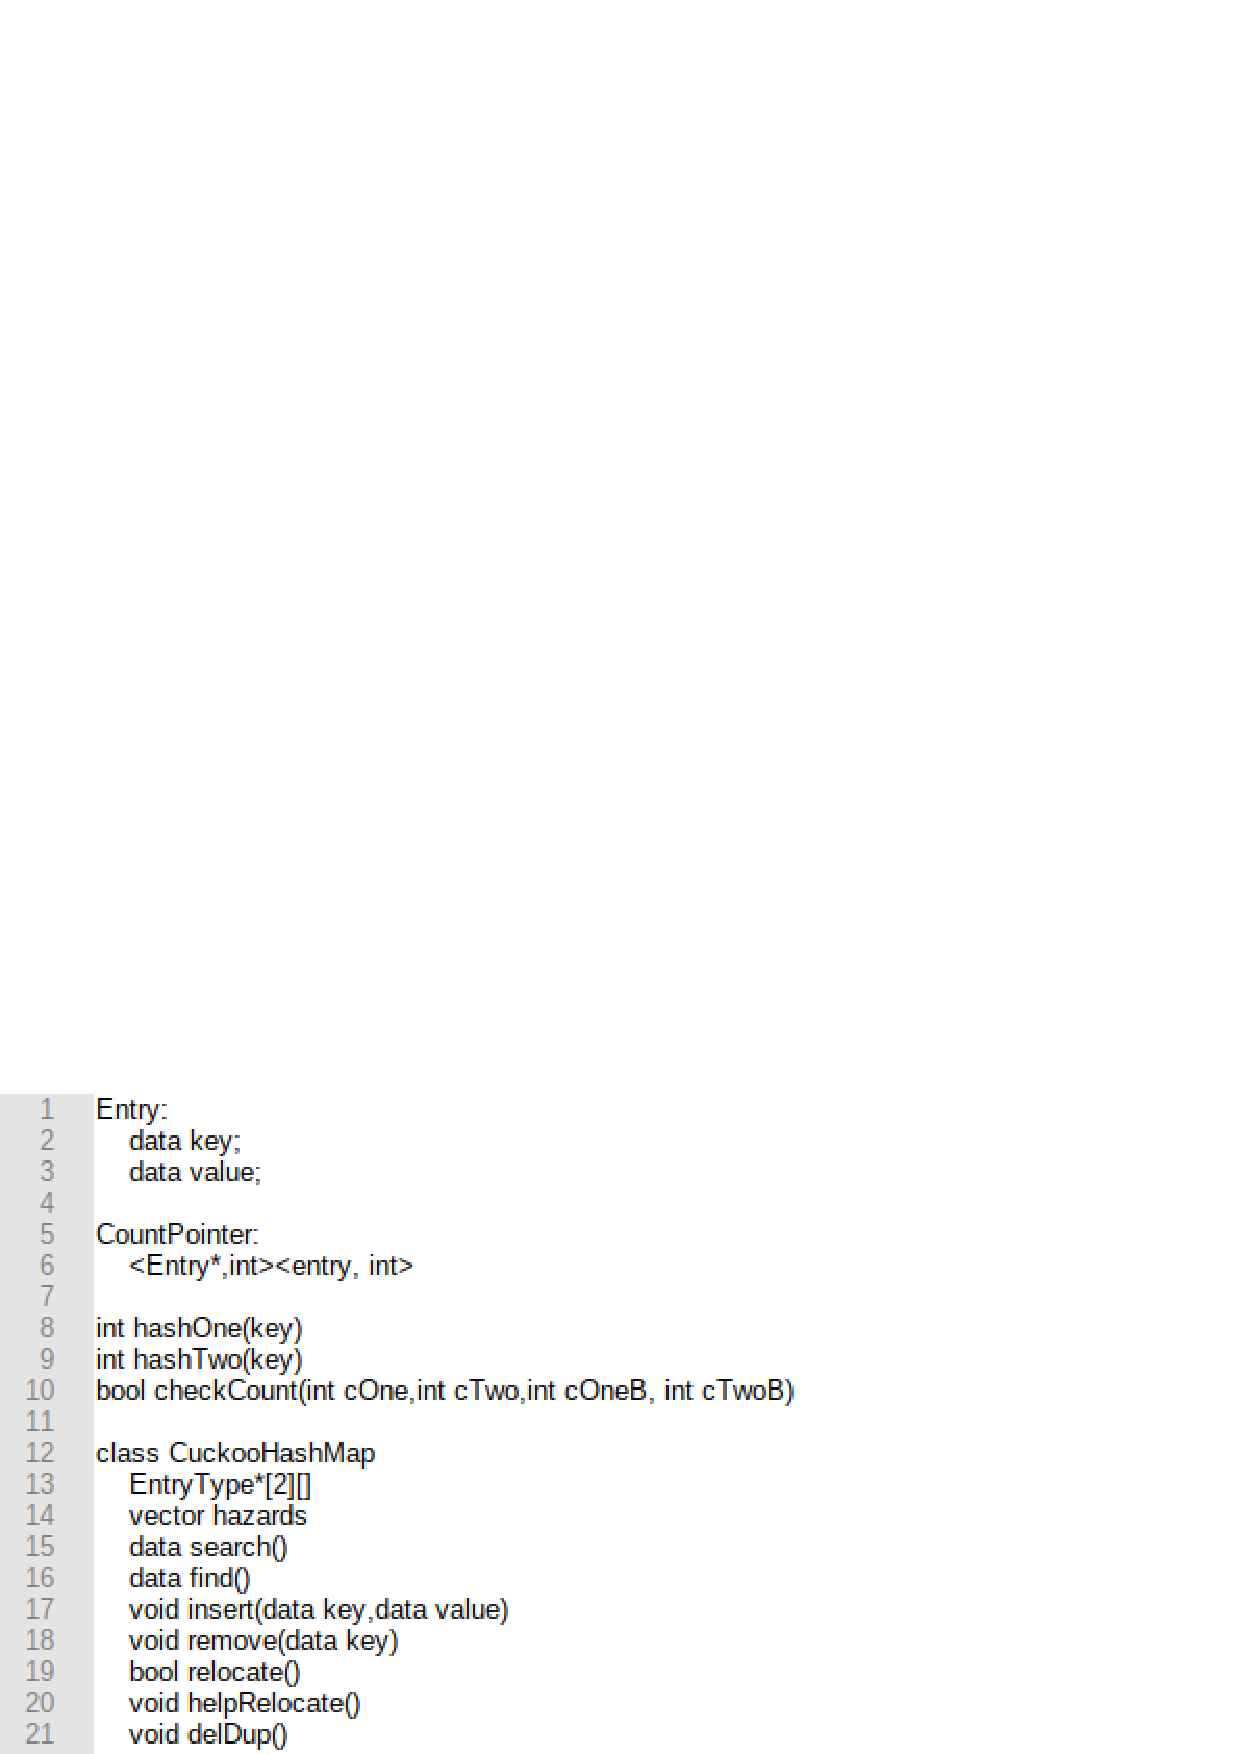
\includegraphics[width=2.7638in,height=3.661in]{Report-img001.png} 
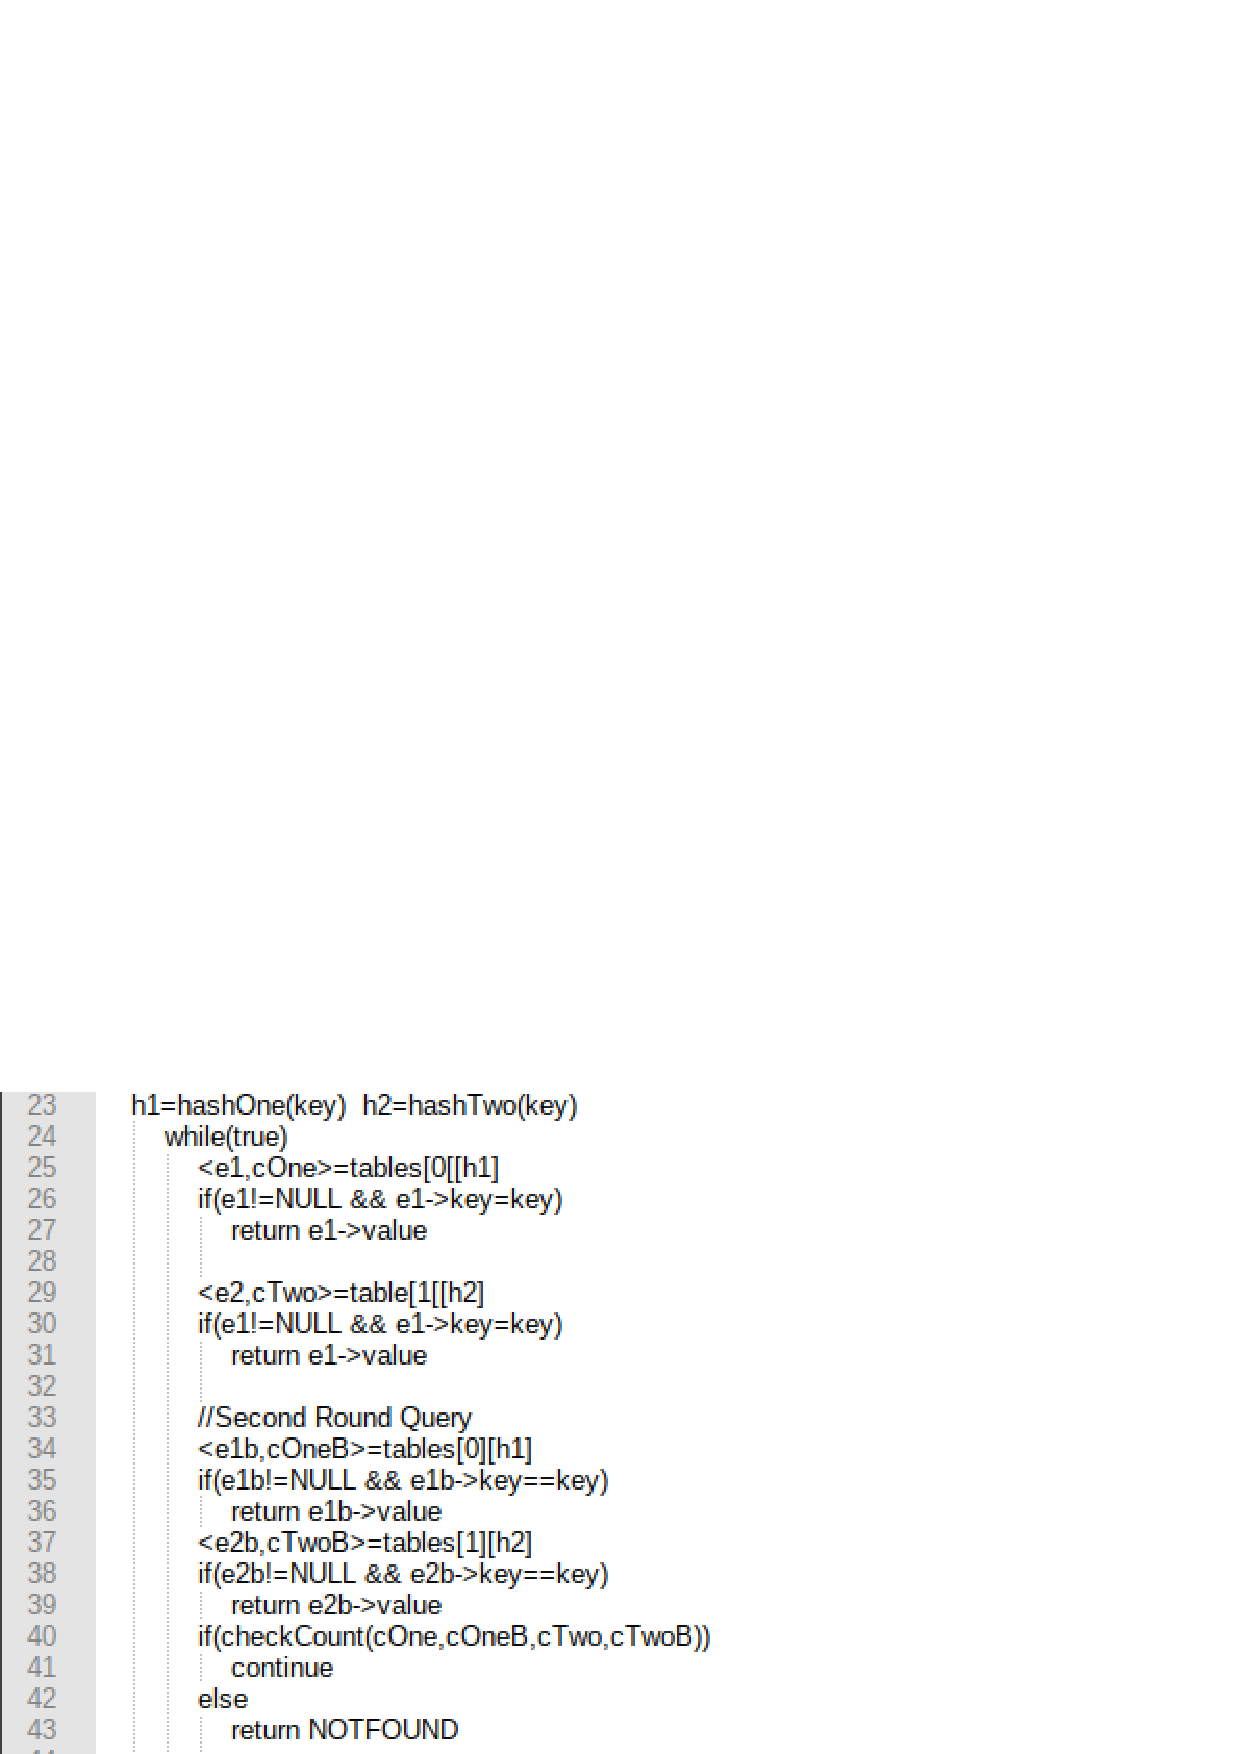
\includegraphics[width=3.2299in,height=2.9598in]{Report-img002.png} }
\begin{center}
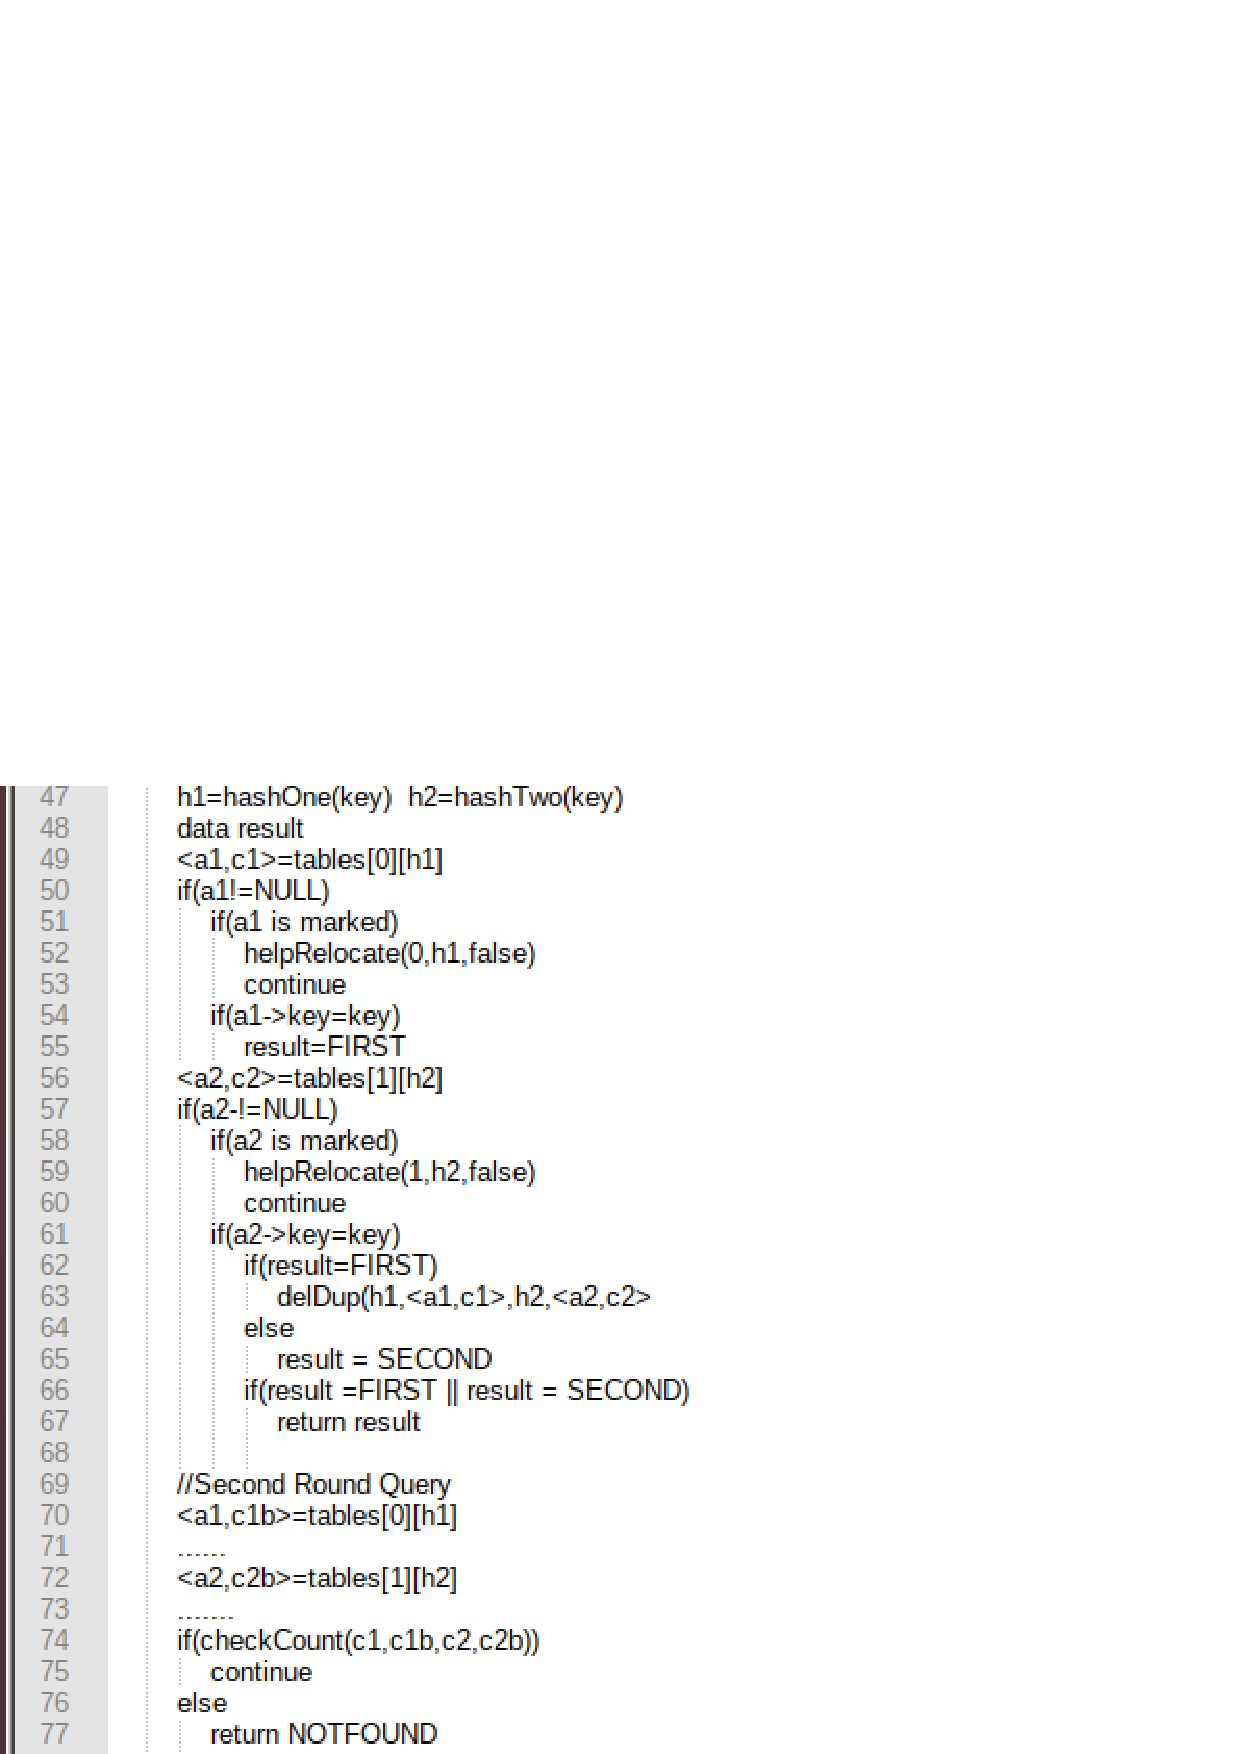
\includegraphics[width=3.278in,height=2.6984in]{Report-img003.png}
\end{center}

\bigskip


\bigskip



\begin{center}
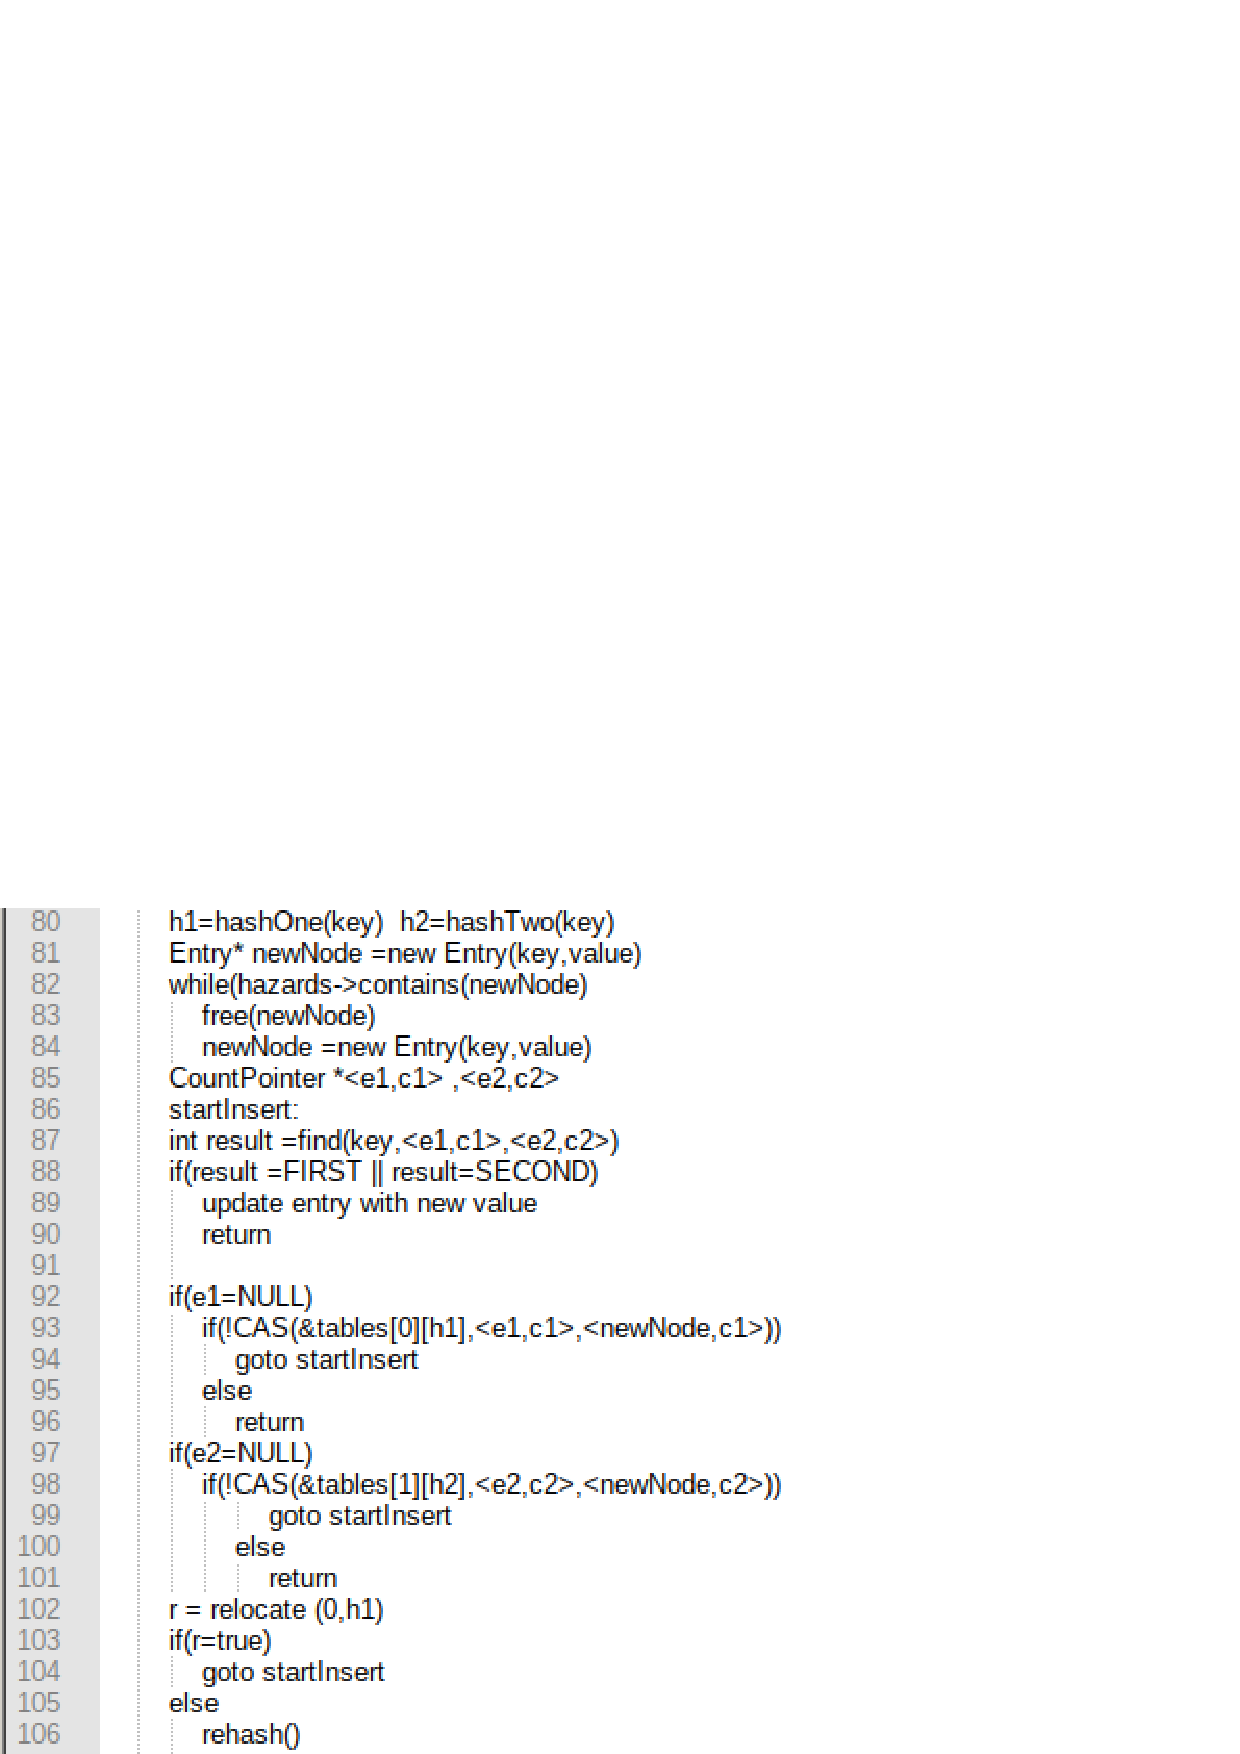
\includegraphics[width=2.7445in,height=2.9634in]{Report-img004.png}
\end{center}
\begin{center}
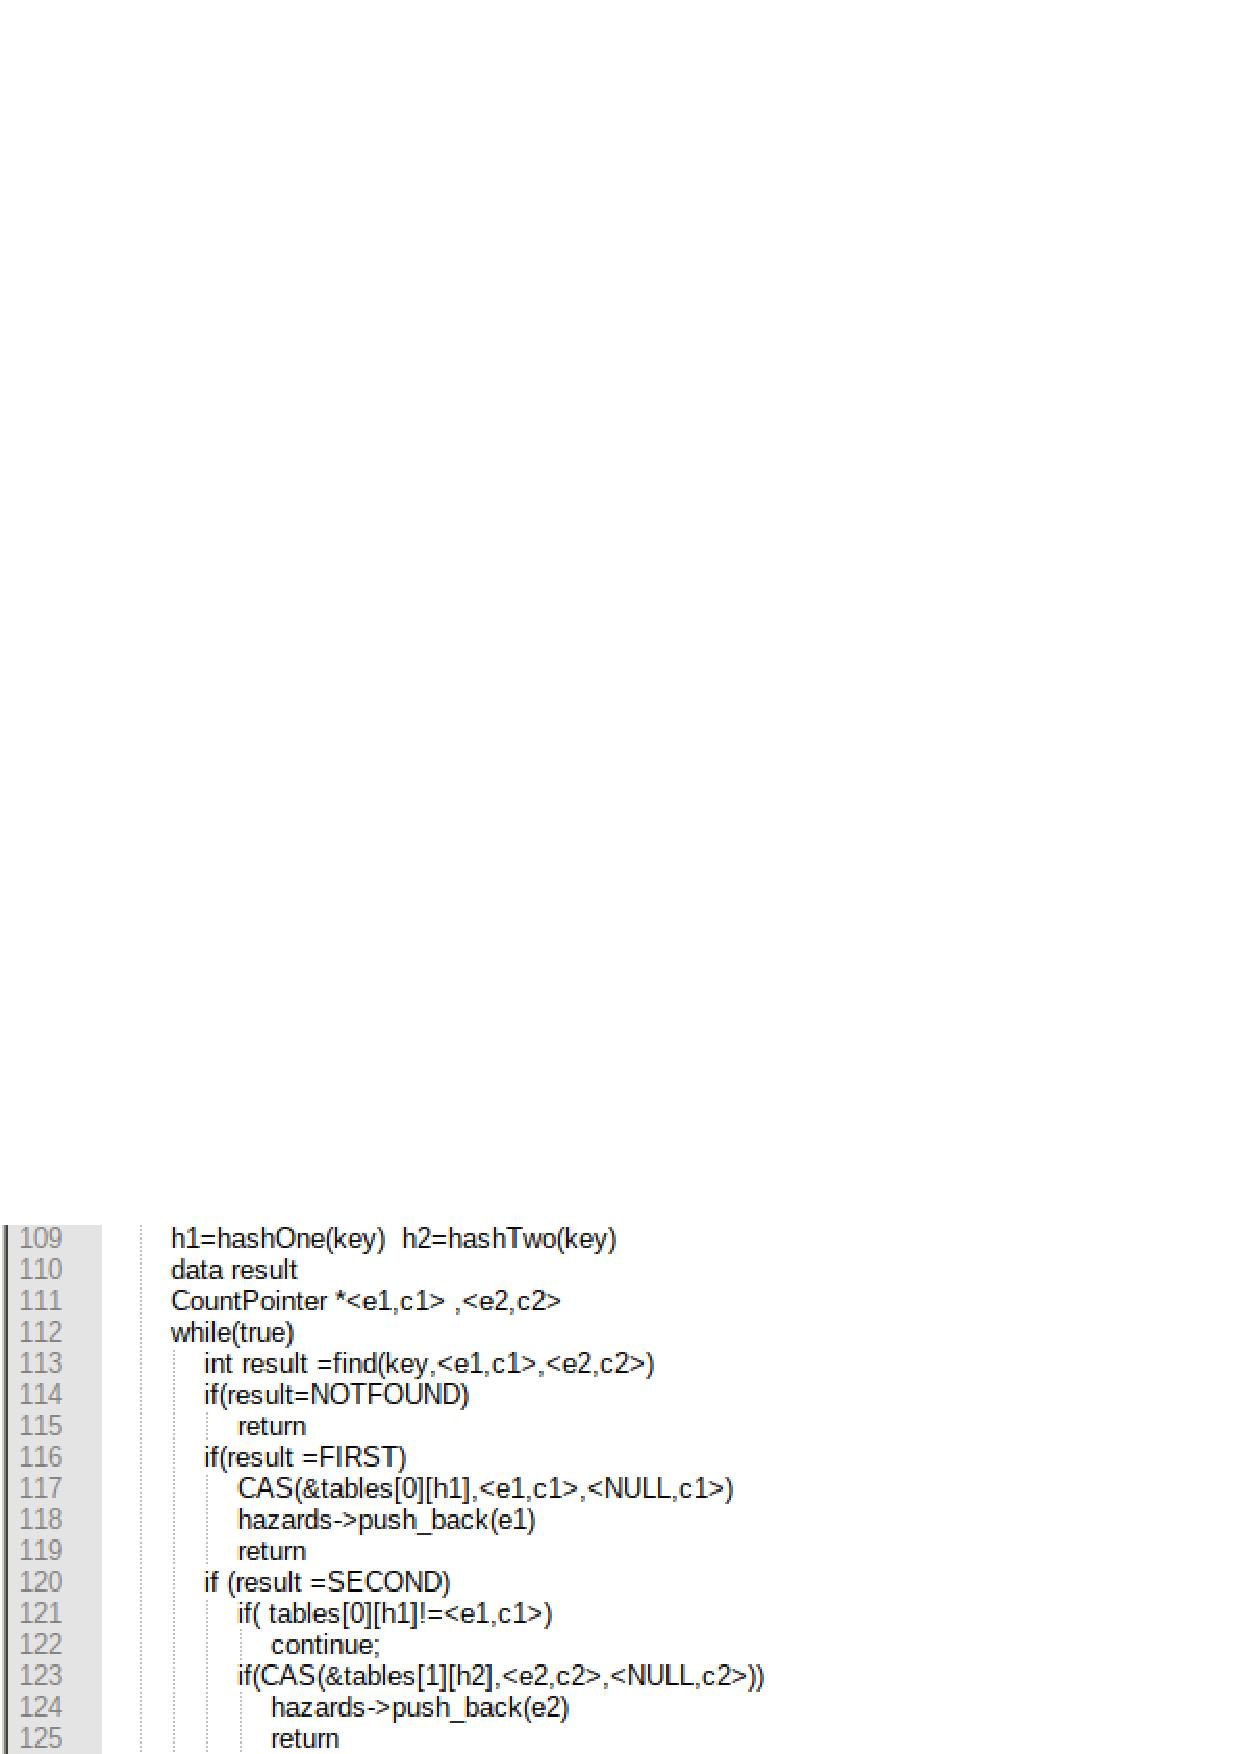
\includegraphics[width=3.9791in,height=2.6457in]{Report-img005.png}
\end{center}

\bigskip


\bigskip


\bigskip


\bigskip


\bigskip


\bigskip


\bigskip


\bigskip


\bigskip


\bigskip


\bigskip

 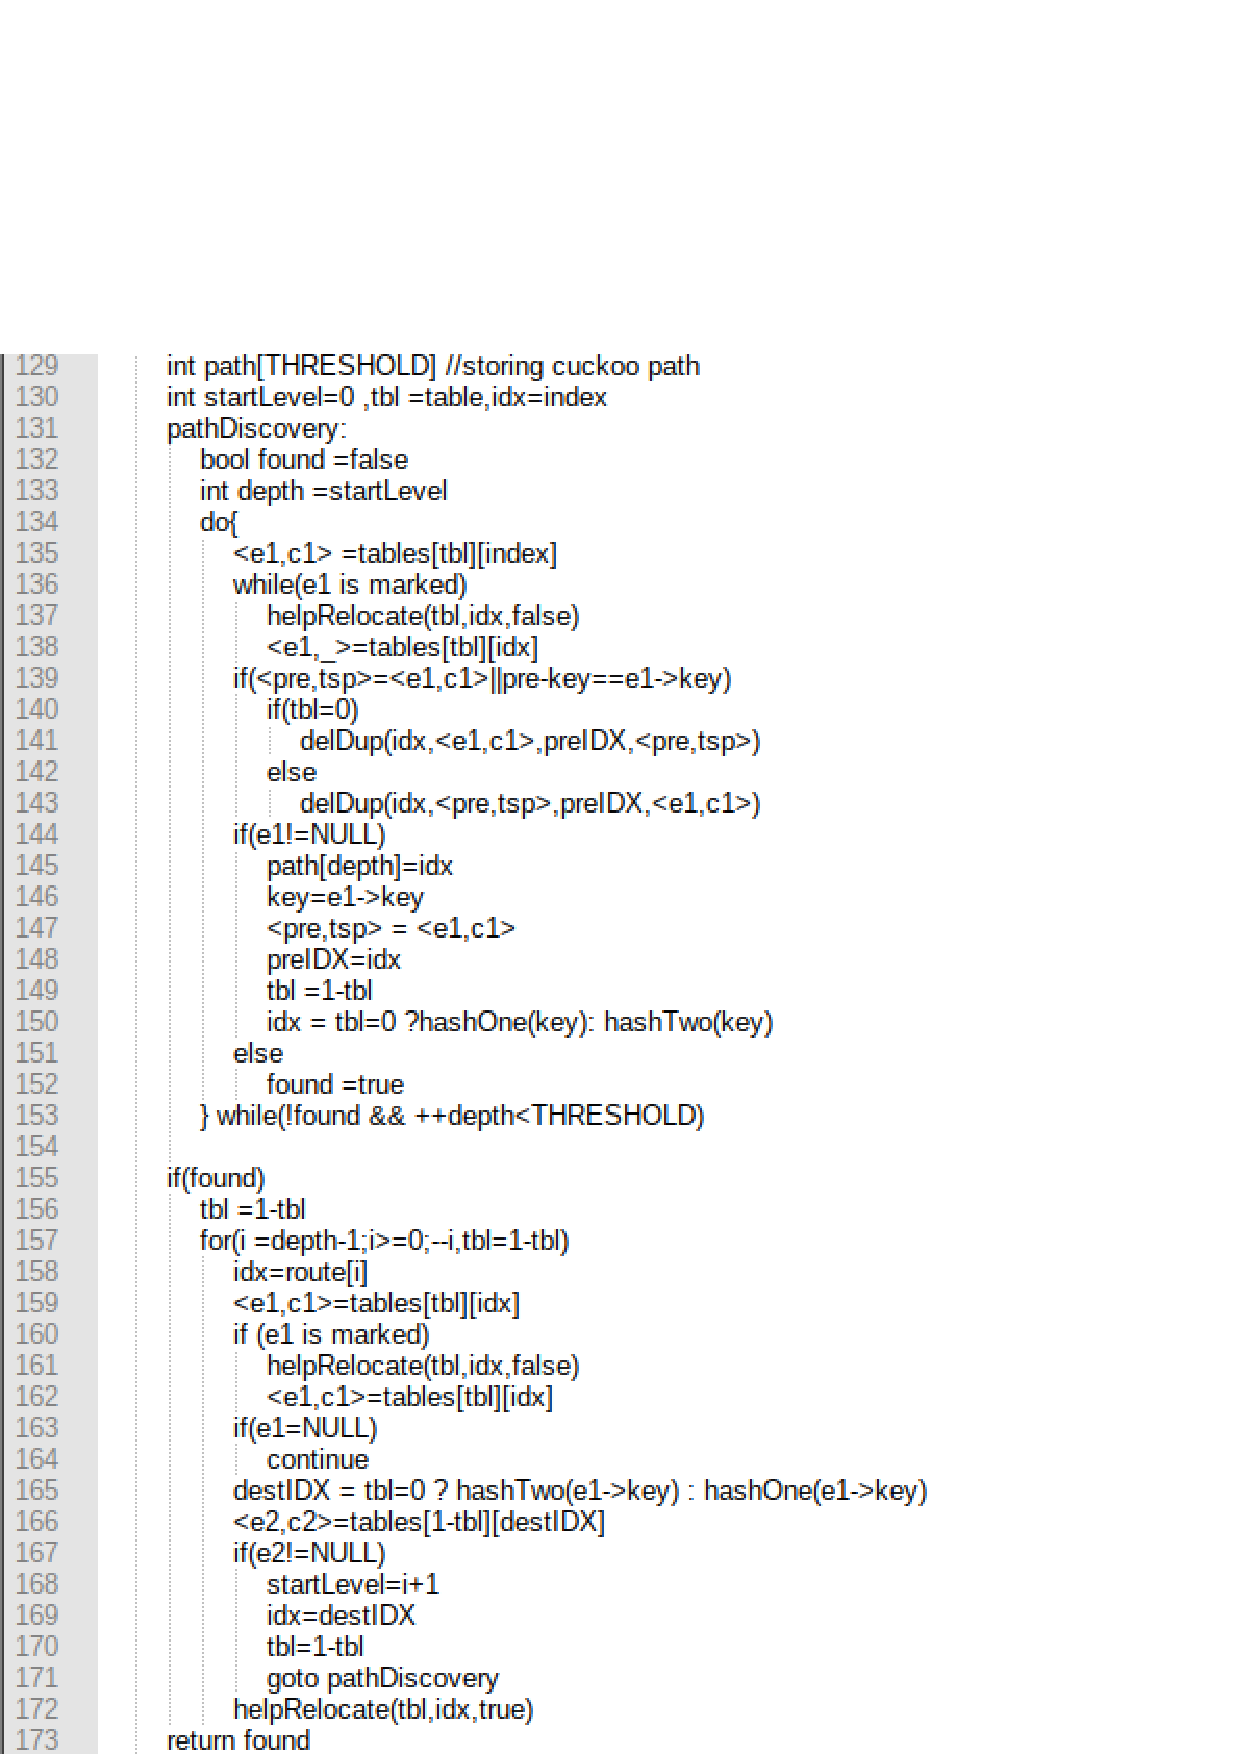
\includegraphics[width=4.9583in,height=0.802in]{Report-img006.png} 

\begin{center}
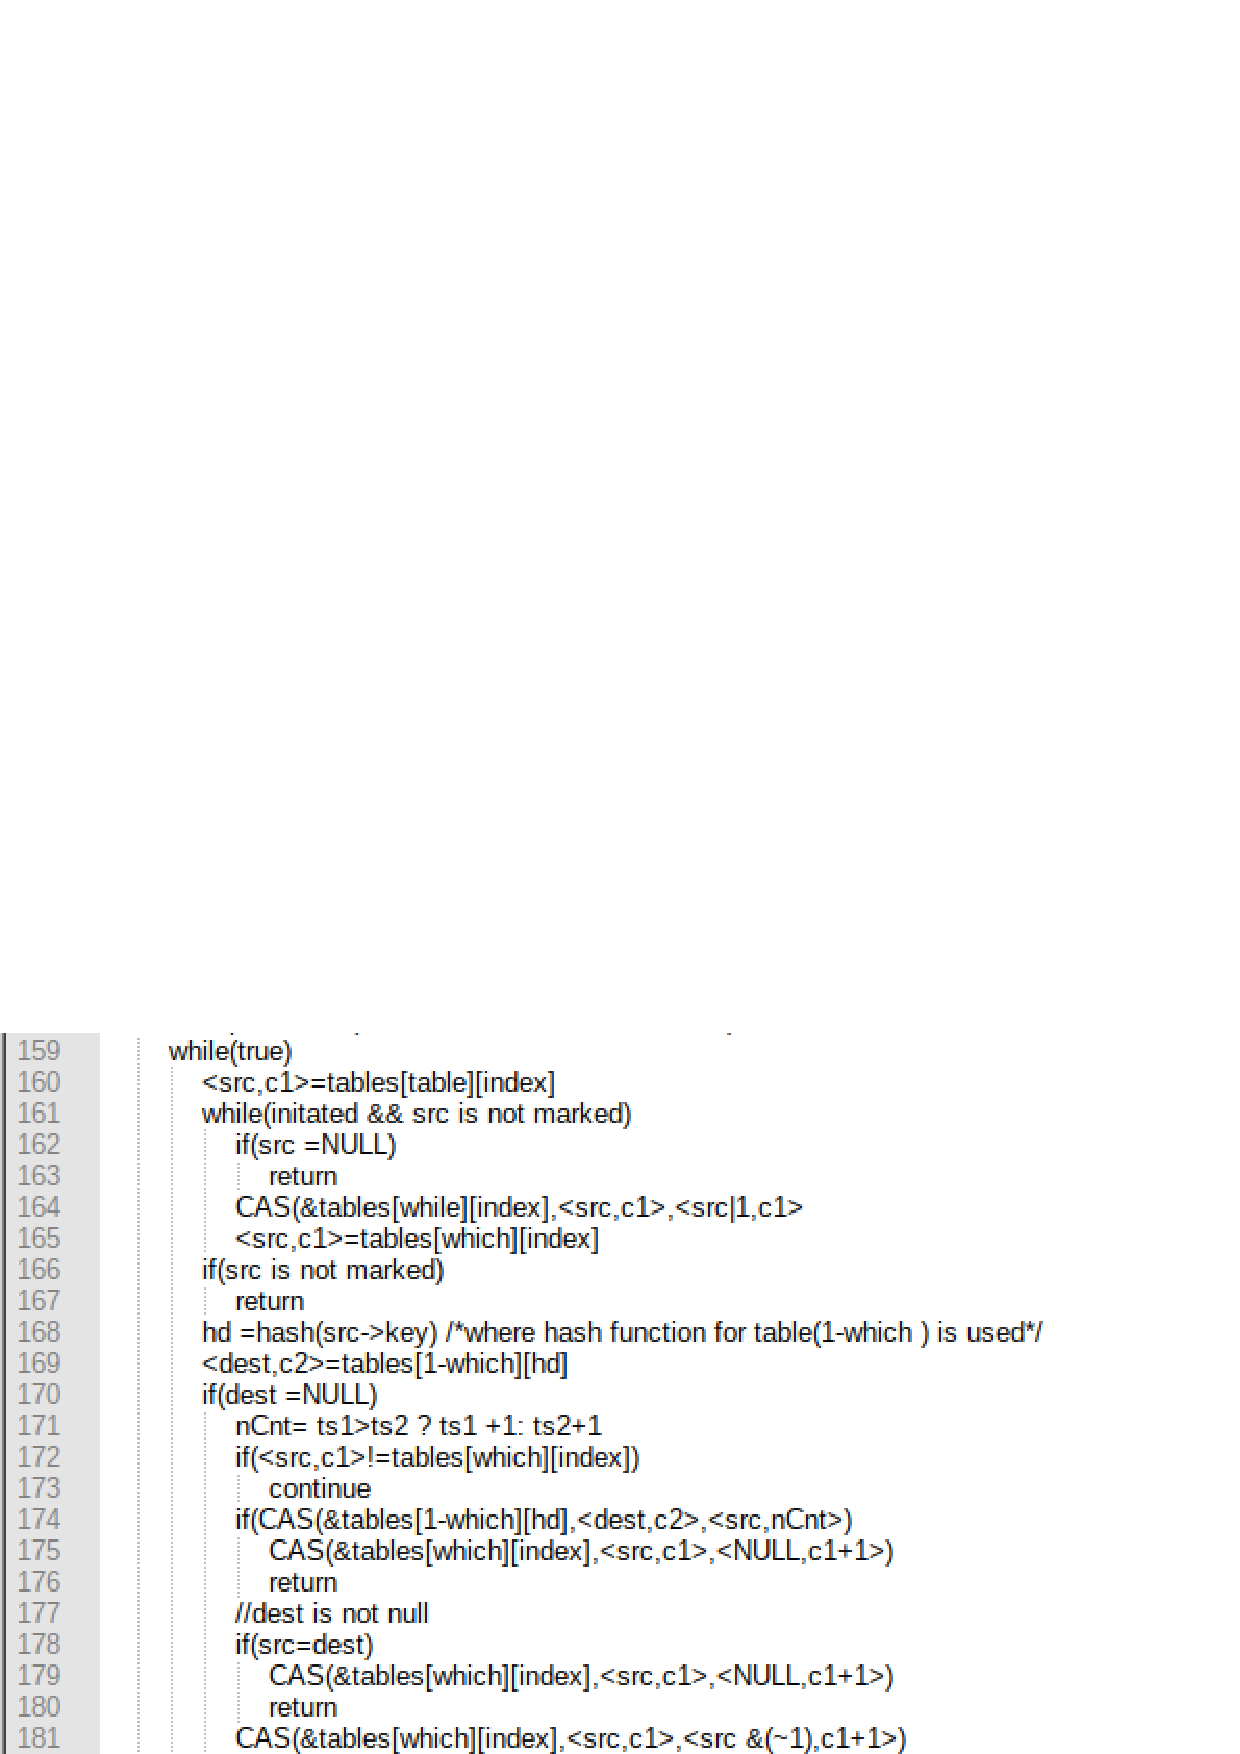
\includegraphics[width=4.052in,height=2.7071in]{Report-img007.png}
\end{center}
\begin{center}
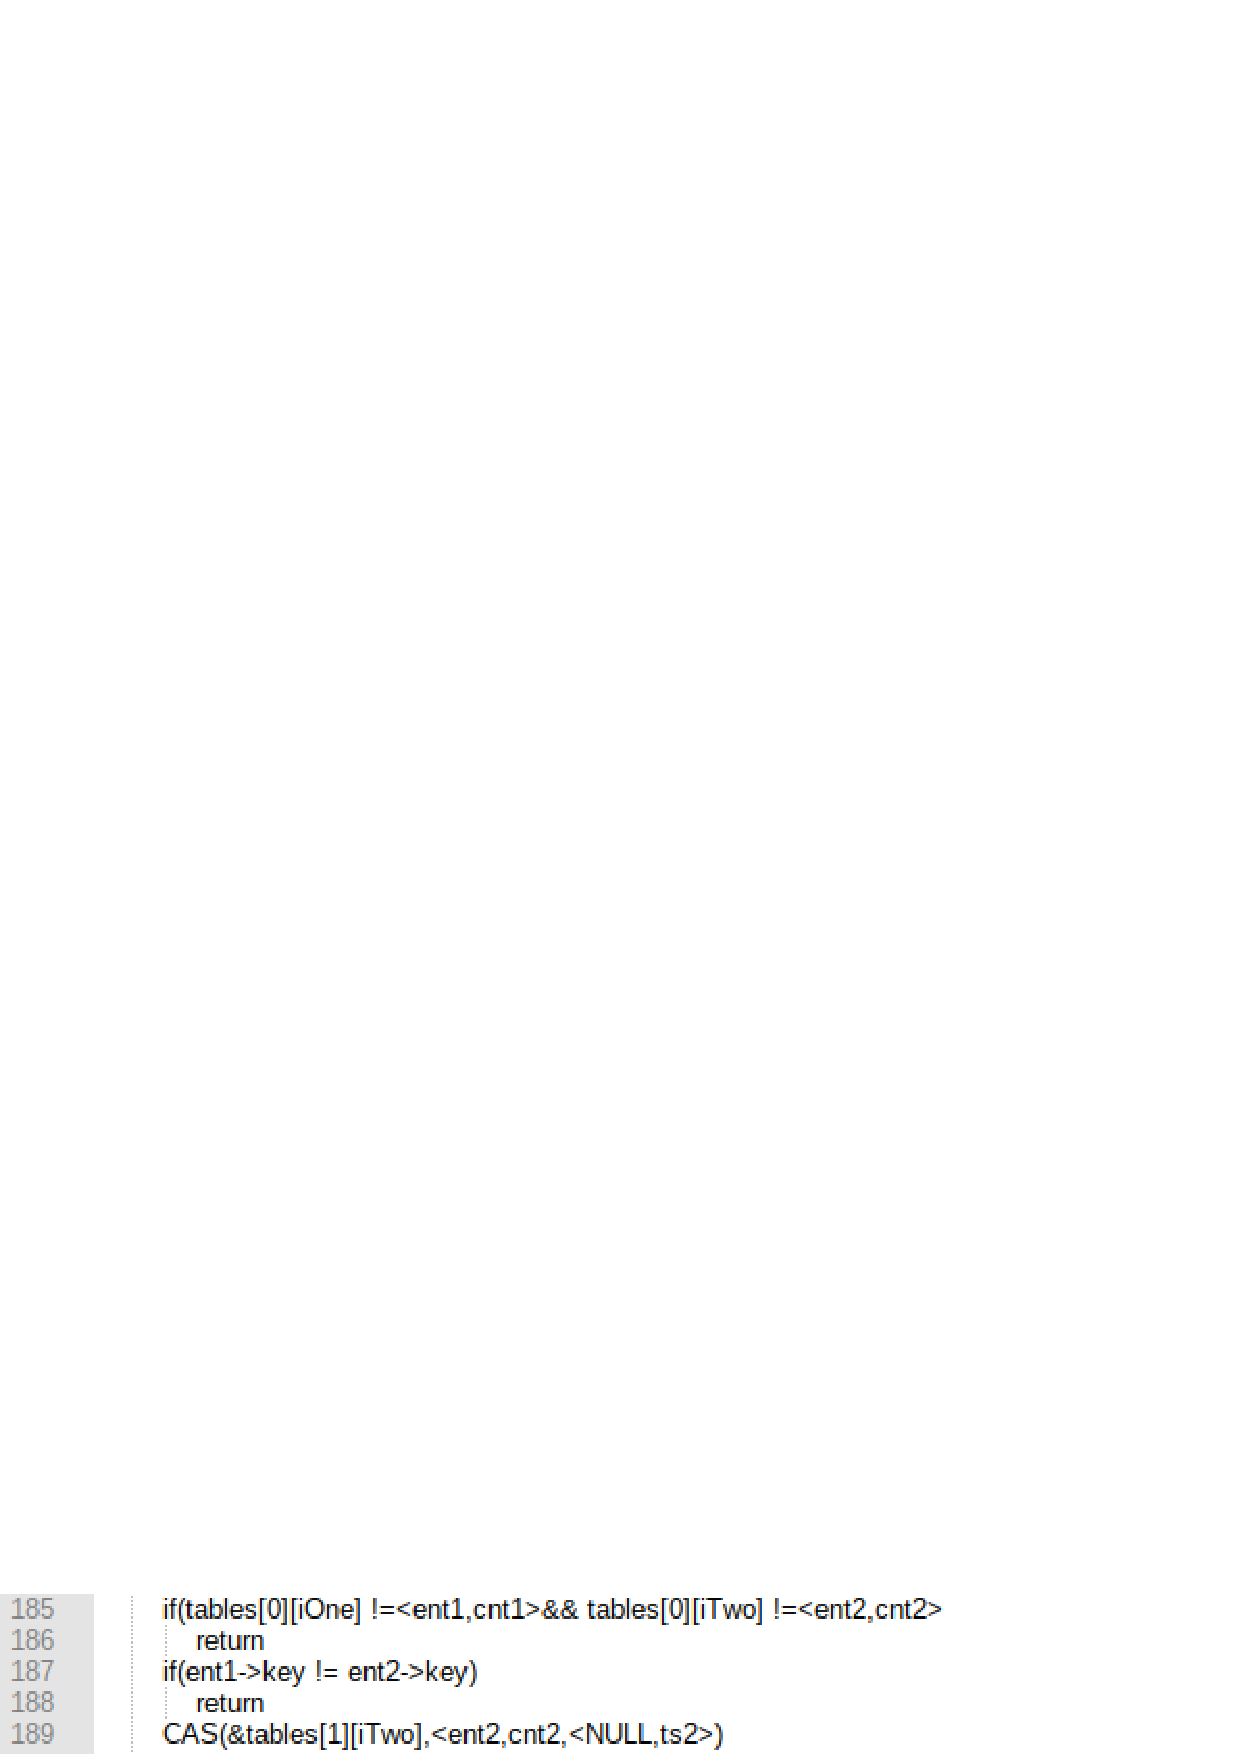
\includegraphics[width=2.7917in,height=4.1783in]{Report-img008.png}
\end{center}
\subparagraph[Program 1: Search(data key)]{Program 1: Search(data key)}

\bigskip

The search operation starts with the first-round query by reading the slots in tables [0] (lines 25-7) and the tables
[1] (lines 29-31). If the key is round is either of these slots, the value mapped to key is returned. As previously
mentioned, this can miss a key being actively relocated. To combat this, a second round is added to the query
operation. This two-round query can still miss a key being constantly relocated between the two tables. To mitigate
this, a technique based on Lamport's logical clocks [8]. The idea is to attach a counter to each slot of the table.
Both the slot's address and counter can be read in one step. The disadvantage of this technique is that the counter
which has been increased by 216 + k can be misinterpreted to be increased by just k, where k is any counter value.
However, such an increment of 216 + k can only be made by many thousands of relocation operations happening at the same
slot. Moreover, it must have happened in a very short period of time of a search operation to cause such
misinterpretation. With a good choice of hash functions, the possibility that such misinterpretation happens is
practically impossible. Therefore, 16 bits are enoughProgram 2: Locate (data
key,CountPointer{\textless}a1,c1{\textgreater},CountPointer{\textless}a2,c2{\textgreater}

Program 2 shows the pseudo code of the locate operation, which functions similarly to the search. The locate takes an
argument key and answers if, and in which sub-table, the key exists. In addition, it also reports the current values
stored at the two possible positions of key. The logic flow of the locate is similar to that of the search, in the
sense that it also uses a two-round query. However, it has 3 main differences compared to the search. First, if it
reads an entry who LSB is marked, indicating an on-going relocation operation, it helps the operation (lines 51-52, and
58-59). Secondly, it examines both sub-tables instead of returning immediately when key is found. This is to discover
if two instances of the key exist in two sub-tables. When the same key is found on both sub-tables, the one in the
second sub-table tables[1] is deleted (line 63), as described in Section II. Finally, locate returns also current items
which are stored at two possible slots where the key should be hashed to. This information is used by the invokers,
such as insert and remove.

\subparagraph{Program 3: Insert (data key, data value)}

\bigskip

The insert starts by invoking locate at line 87. If the key is found in either of the sub tables, the key is updated
with the new value. Otherwise, the procedure to begin the key begins. If either of the two slots (lines 92 and 97) are
empty the key will be inserted by a CAS. If both slots are occupied, a relocation operation is triggered. The relocate
operation is further described in Program 5. If the relocation succeeds, the insertion is reattempted, Otherwise, the
relocation path's length exceeded the threshold and the relocation failed. \ In this case either a rehashing of the
table or a resizing of the tables is needed.

\subparagraph{Program 4: Remove (data key)}

\bigskip

The remove operation also starts by invoking locate at line 101. If the key is found, it is removed by a CAS, either at
line 117 or 123.

\subparagraph{Program 5: Relocate (int table, int index)}

\bigskip

When both slots which can accommodate a newly inserted key are occupied by existing keys, one of them is relocated to
make space for the new key. First, the cuckoo path is discovered, lines 114-136. Then, the empty slot is moved
backwards to the beginning of the path, where the new key

is to be inserted, lines 155-172. 

The path discovery starts from a slot index of one of the sub-tables identified by which and runs at most THRESHOLD
steps along the path. If table[table][index] is an empty slot, the discovery is finished (line 172). Otherwise, the key
should be relocated to its slot in the other sub-table. The discovery then continues with the other slot of key. If
this slot is empty, the discovery finishes. Otherwise, the discovery continues as before. Each element along the path
is identified by a sub-table and an index on that sub-table. Along the path, the sub-tables that elements belong to
alternatively change between the first and second ones. Therefore, the data of the path which need to be stored are the
indexes of the elements along the path and the sub-table of the last element.

Once the cuckoo path is found, the empty slot is moved backwards along the path by a sequence of swaps with the
respective preceding slot in the path. Each swap is actually a relocation of the key in \ \ the source, to the
destination. Because of the concurrency, the entry stored in the source might have changed. So, the relocation
operation needs to update the destination and check for its emptiness (lines 168-9), and retry the path discovery if
the destination is no longer empty (line 171). If the destination is still empty, the relocation is performed in three
steps.

\subparagraph{Program 6: Help Relocate (int table, int index, bool initiated)}

\bigskip

First, the source entry's LSB is marked to indicate the relocation intention (line 164). Then, the entry is copied to
the destination slot (line 174), which has been made empty. Finally, the source is deleted (line 175). Marking the LSB
allows other threads to help the on-going relocation, for example at lines 136 and 51.

After a slot is marked to aid relocation, the destination of the relocation may have been altered and is no longer
empty. This can be because of one of two things. Either the key may have already been relocated by another thread or a
concurrent insertion has inserted a new key to that destination slot. In the case of the former (line 174), the source
of the relocation is deleted either by that helping thread (line 175) or by the current thread (line 178). If it is the
latter case, the help relocation fails, unmarks the source (line 181) and returns. The relocation process then
continues but will most likely have to retry the path discovery in the next loop.

Program 7: Delete Duplicate (int iOne, CountPointer{\textless}ent1, cnt1{\textgreater},int iTwo,
CountPointer{\textless}ent2, cnt2{\textgreater}


\bigskip

\ \ The delete duplicate operation starts by verifying the two slots are still equal. It then checks if the keys are
equal. The key in the second table is then remove by way of a compare and swap.

\section[Proof of Correctness]{Proof of Correctness}
This section will be dedicated to proving that this hash table is both linearizable and lock free. To start, the
linearizability of the tables will be proven given a key only exists in one sub-table. Next, the linearizability will
be proven if a given key exists in both tables. Then lock-freedom will be proven. In the following, it is presumed a
key can be in two possible positions, tables[0][h1] and tables[1][h2].

Lemma 1: Search is linearizable.

Proof: search only returns a value when one of the key e, e2, e1b, e1c has an element that matches the key being
searched for and is linearized at that point. The second case is when search returns NOTFOUND.

Lemma 2: The correctness of the search operation is immune to the physical key being present in both sub tables.

Lemma 3: The search operation finishes after a finite number of steps, or another operation must have finished after a
finite number of steps.

Proof: The search operation has only one while loop which, according to Lemma 1, repeats only when there are relocations
of keys stored in tables [0] [h1] and tables[1][h2] . Such relocations mean progress of the respective operations
performing them. This observation holds even when the relocations move keys back and forth between two sub-tables. In
this case, the search might not make progress but the relocation progresses towards the THRESHOLD number of relocation
steps. When it reaches the THRESHOLD and returns false, the insertion calling such a relocation fails and either
rehashes or resizes the hash table.

Lemma 4: This locate operation is linearizable.

Lemma 5: The insert operation is linearizable.

Lemma 6: The remove operation is linearizable.

Lemma 7: A locate operation finishes after a finite number of steps, or another operation must have finished after a
finite number of steps.

Lemma 8: An insert operation finishes after a finite number of steps or another operation must have finished after a
finite number of steps.

Lemma 9: A remove operation finishes after a finite number of steps or another operation must have finished after a
finite number of steps.

Lemma 10: The help relocate operation is guaranteed to finish in a finite number of steps.

Lemma 11: If a help relocation operation finishes but fails to relocate tables[table][index], there must be another
operation making progress during that execution of the help relocation.

Theorem 1: The hashing algorithm is linearizable.

Proof: According to Lemmas 5,6,2 and1, this hash table is linearizable. 

Theorem 2: The hashing algorithm is lock-free.

Proof: According to Lemmas 7,8,9 ,10 ,12, and 3 this cuckoo hash table always makes progress after a finite number of
steps.

\section[Results]{Results}
\subsection{Setup}
This new table will be compared with two other implementations. The first is a lock-based chaining hash table, where
linked lists stored elements hashed to the same bucket. The second is a lock-based hopscotch hashing idea.


\bigskip

This section evaluates the performance of the new hash table and compares is against the current state of the art
tables. All implementations were done in C++ and compiled with the same flags. The experiments were done on a four
core, Intel i5-8250 using 8GB DDR3 RAM. To ensure the tables did not fit into the cache the size of the tables were
approximately 2\^{}23 slots. Each test used the same set of keys for all tables. 

\subsection{Results}
 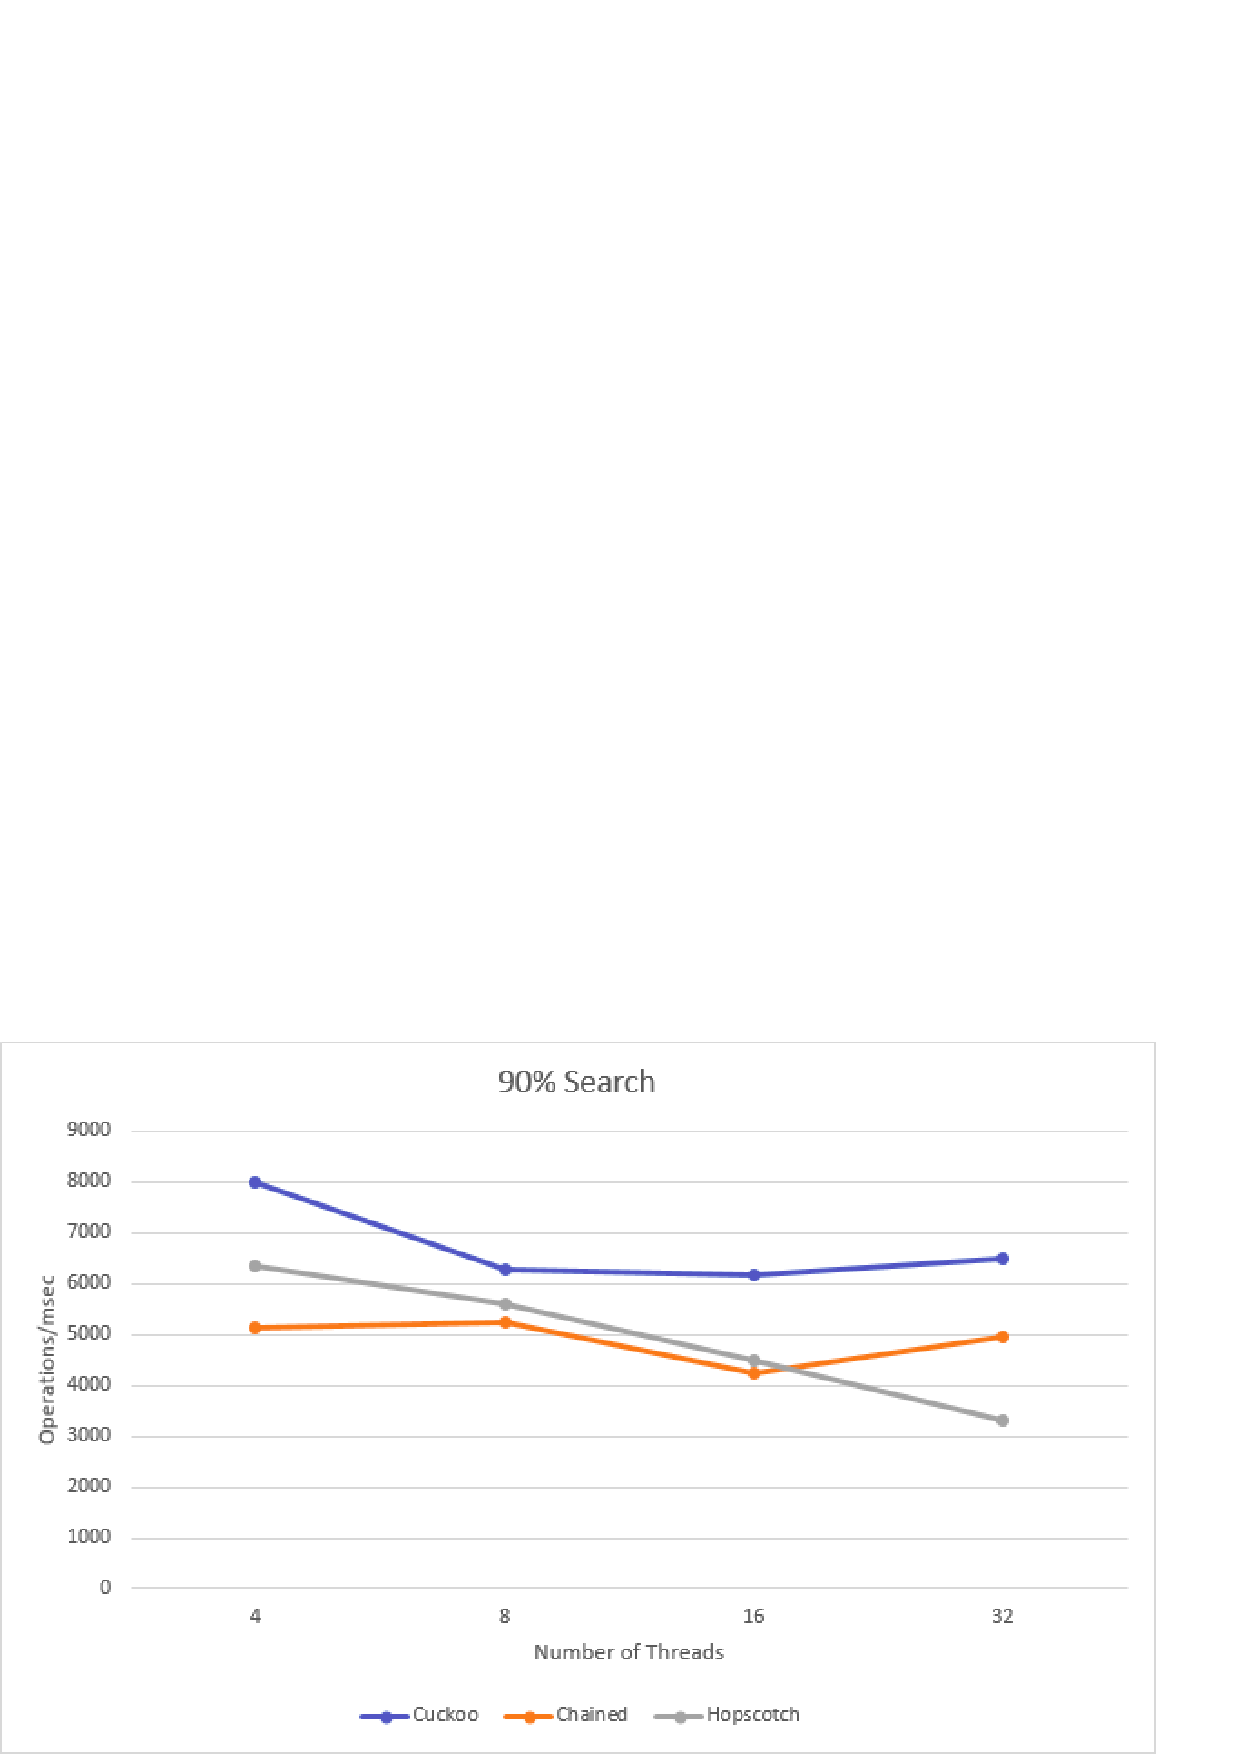
\includegraphics[width=2.9165in,height=1.7453in]{Report-img009.png} 
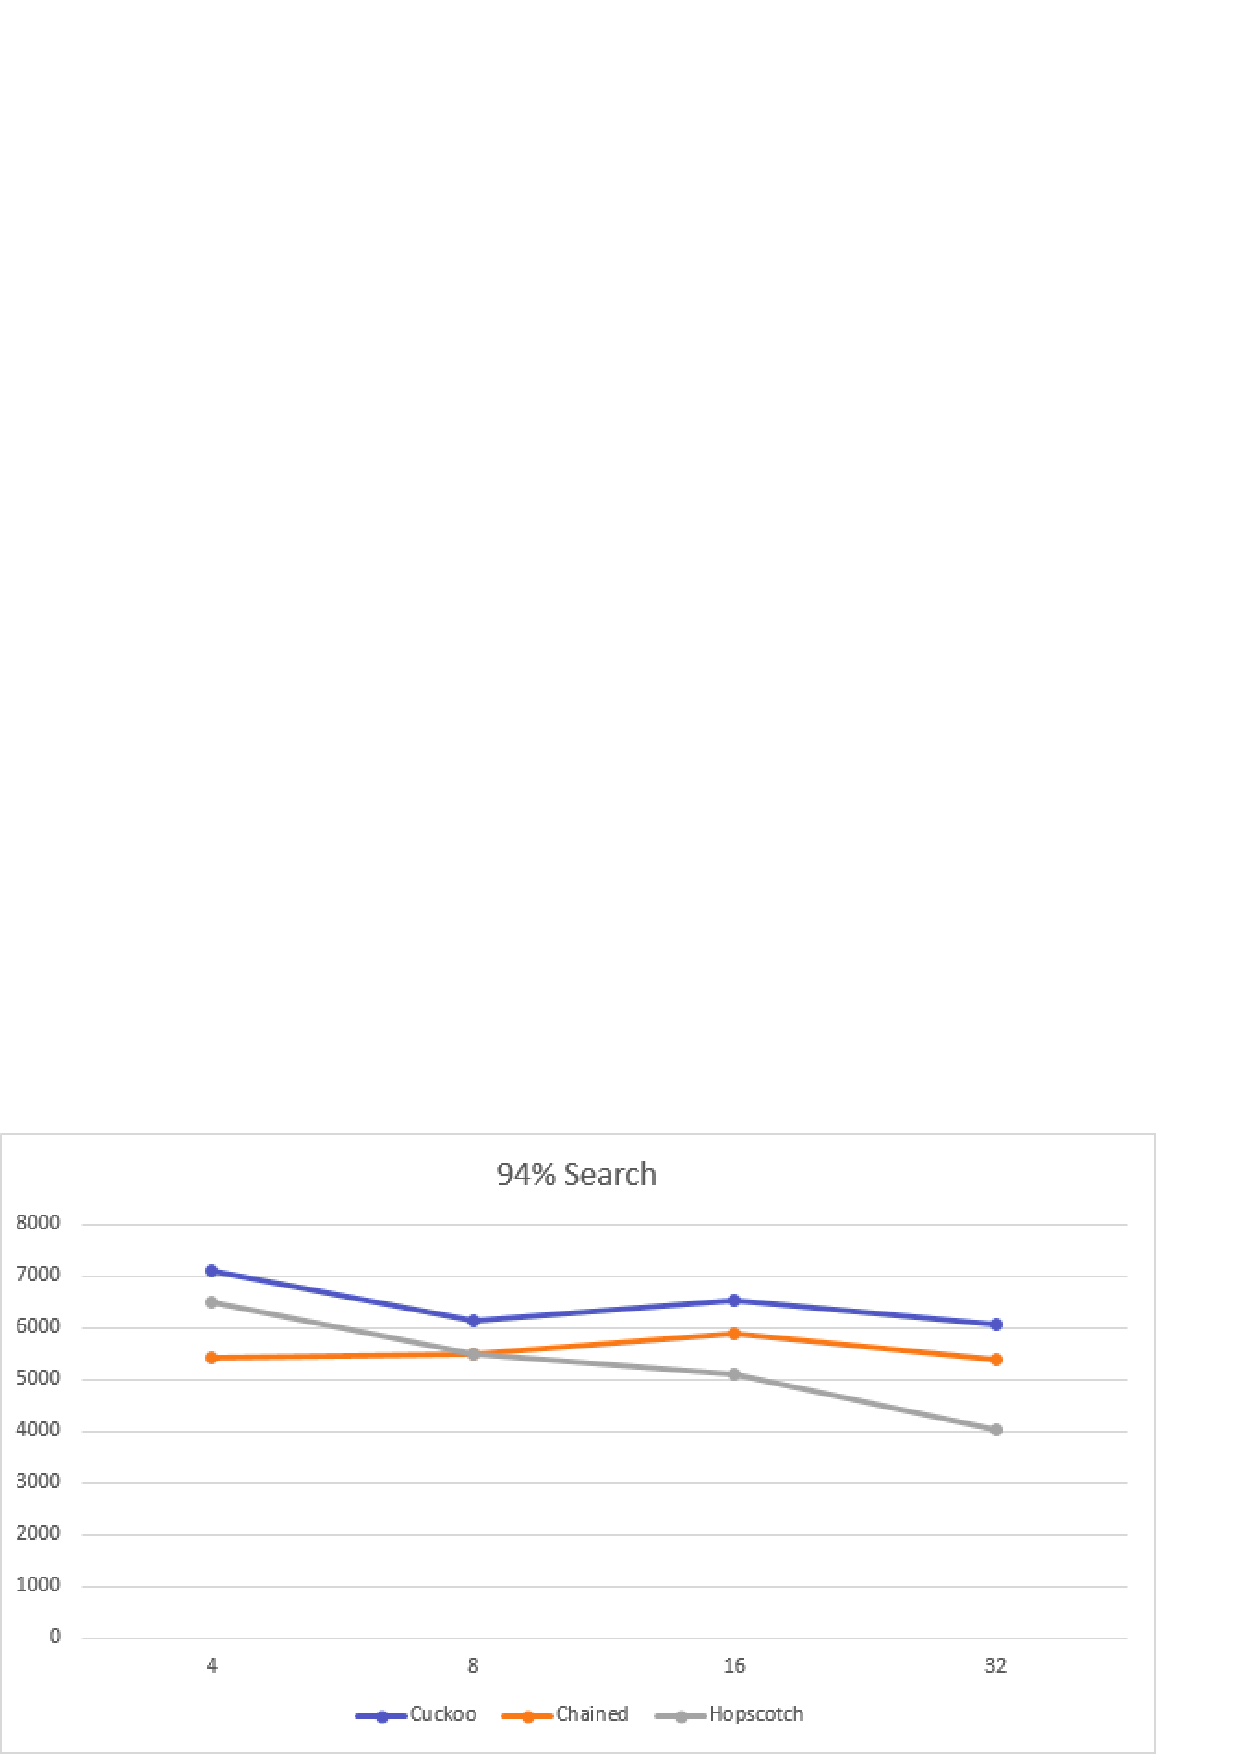
\includegraphics[width=3.0291in,height=1.6783in]{Report-img010.png} 


\bigskip

 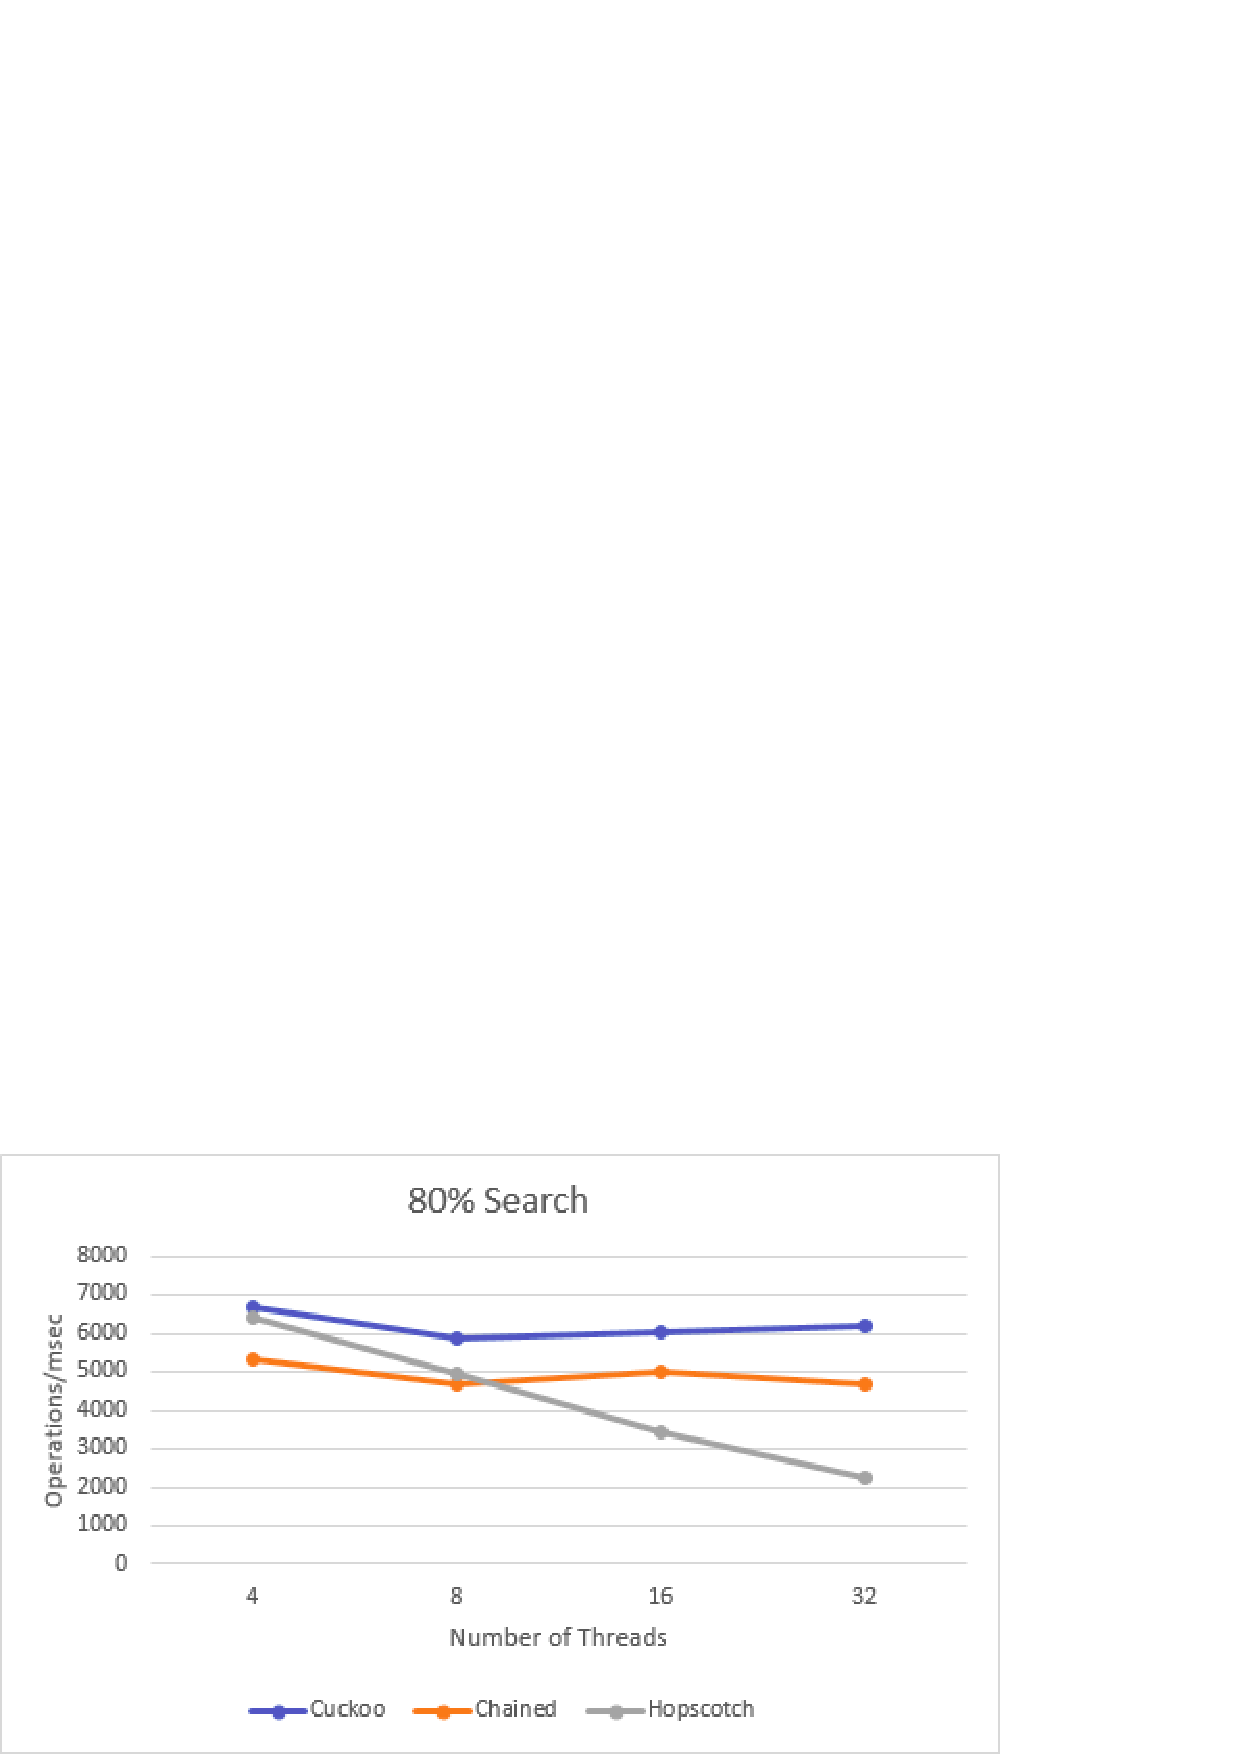
\includegraphics[width=2.6736in,height=1.6043in]{Report-img011.png} 
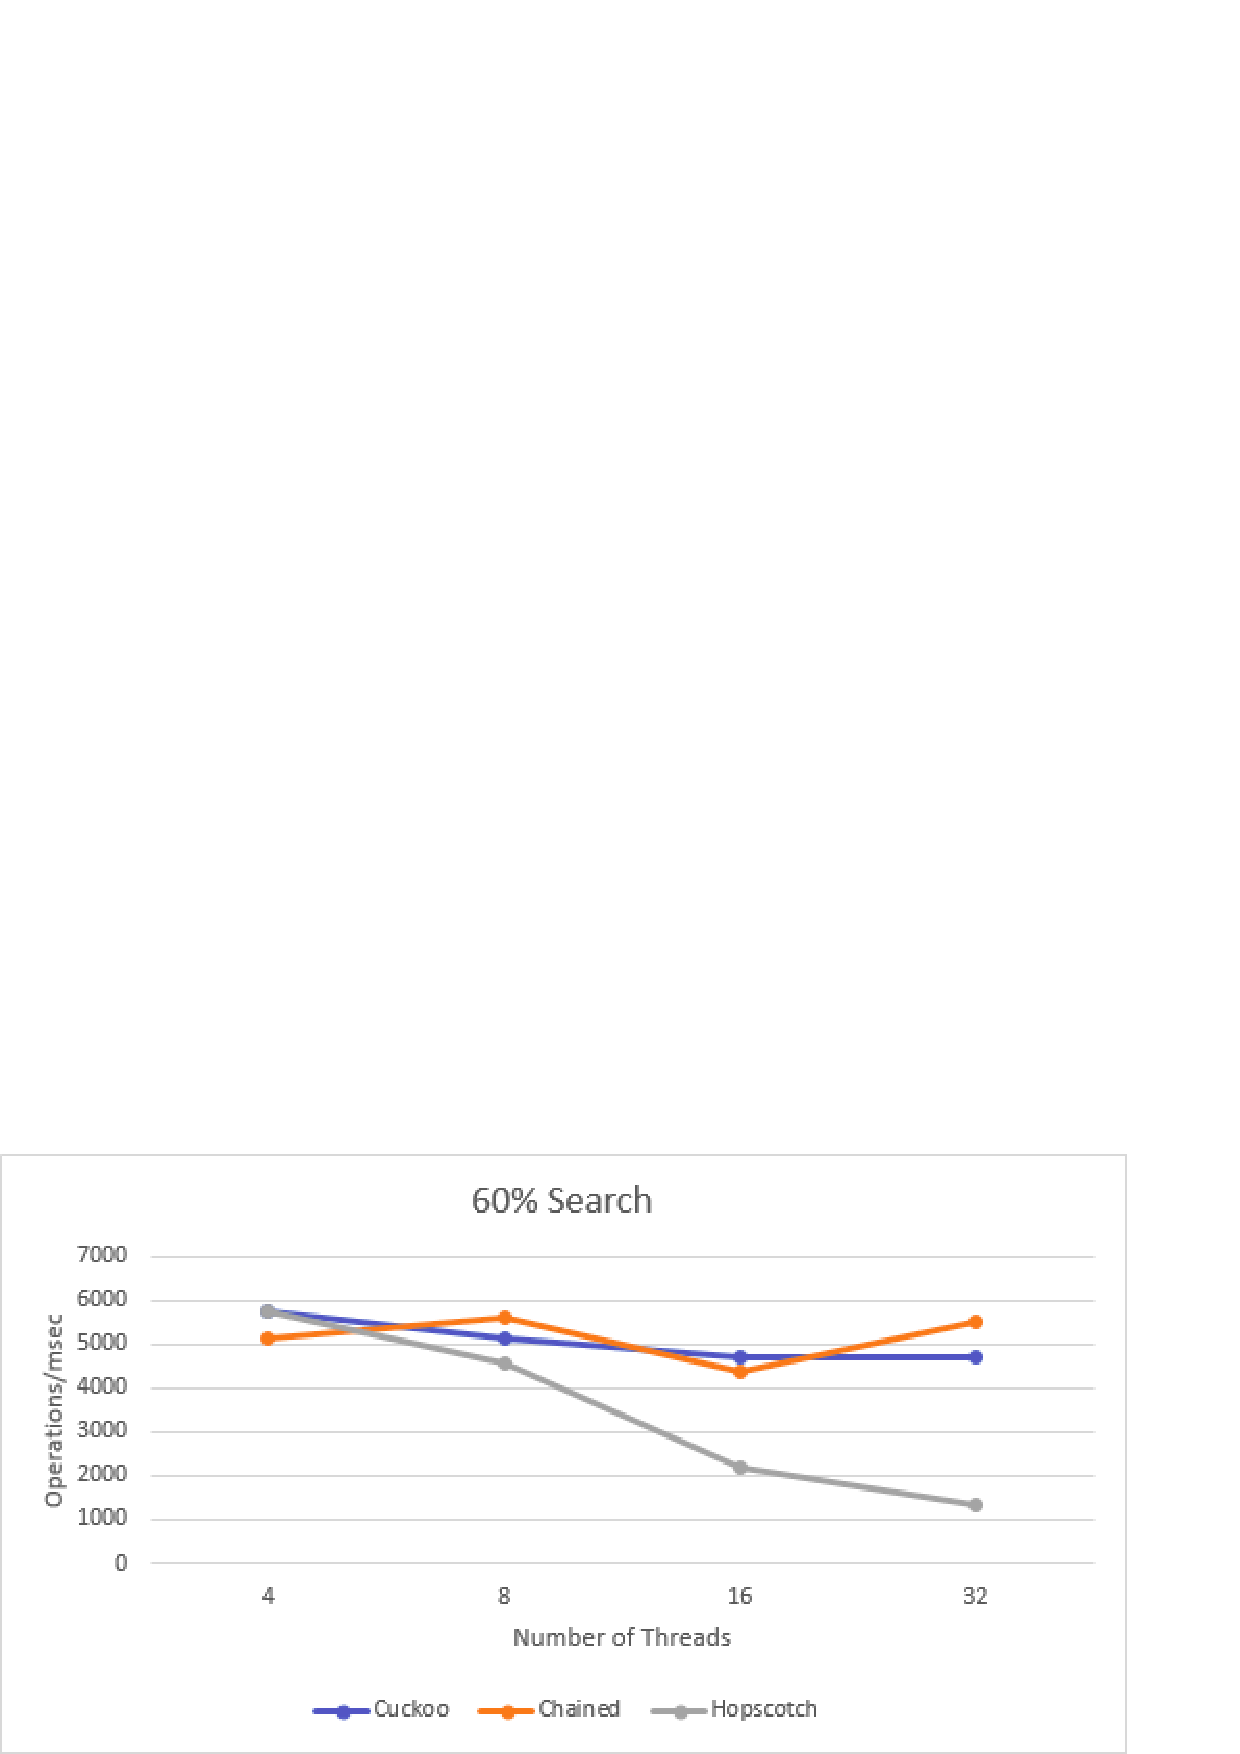
\includegraphics[width=2.9791in,height=1.589in]{Report-img012.png} 

 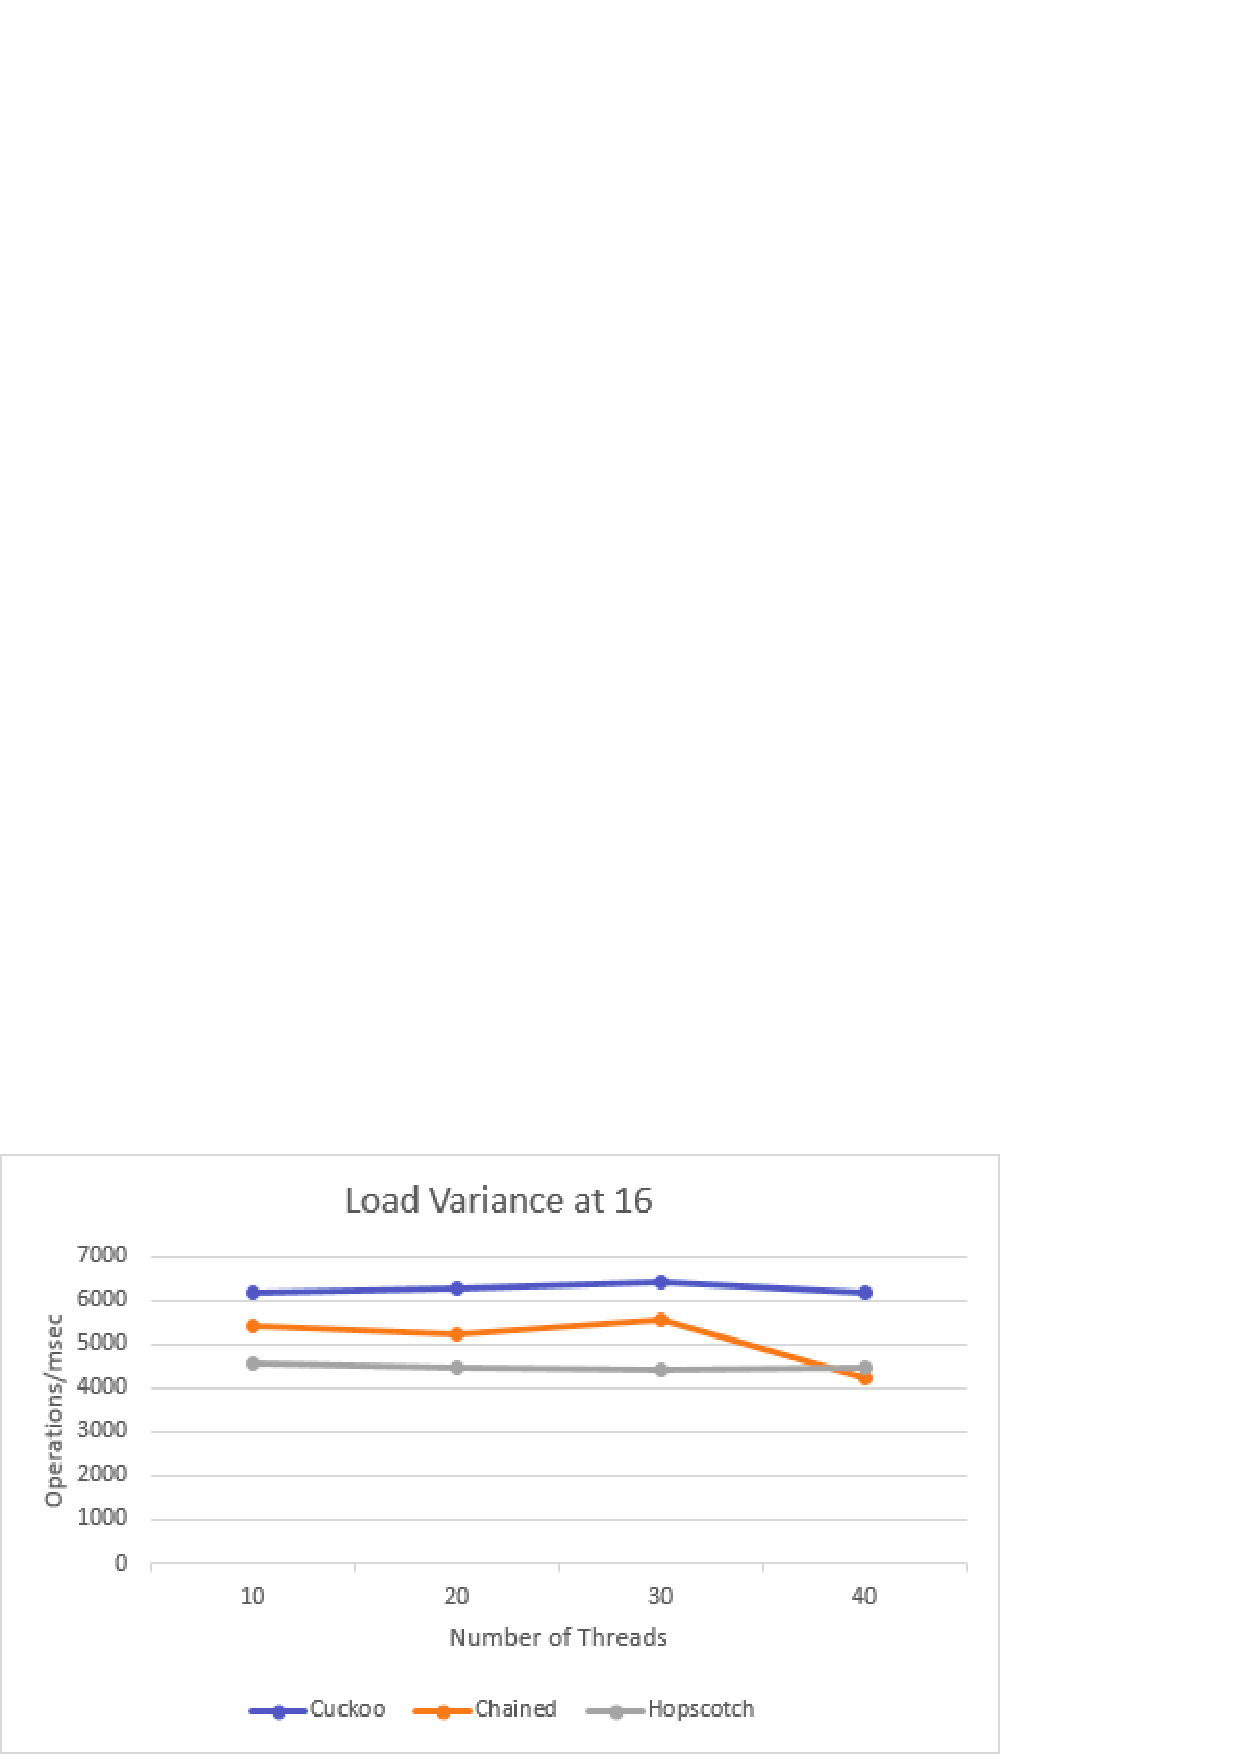
\includegraphics[width=2.9583in,height=1.8083in]{Report-img013.png} 
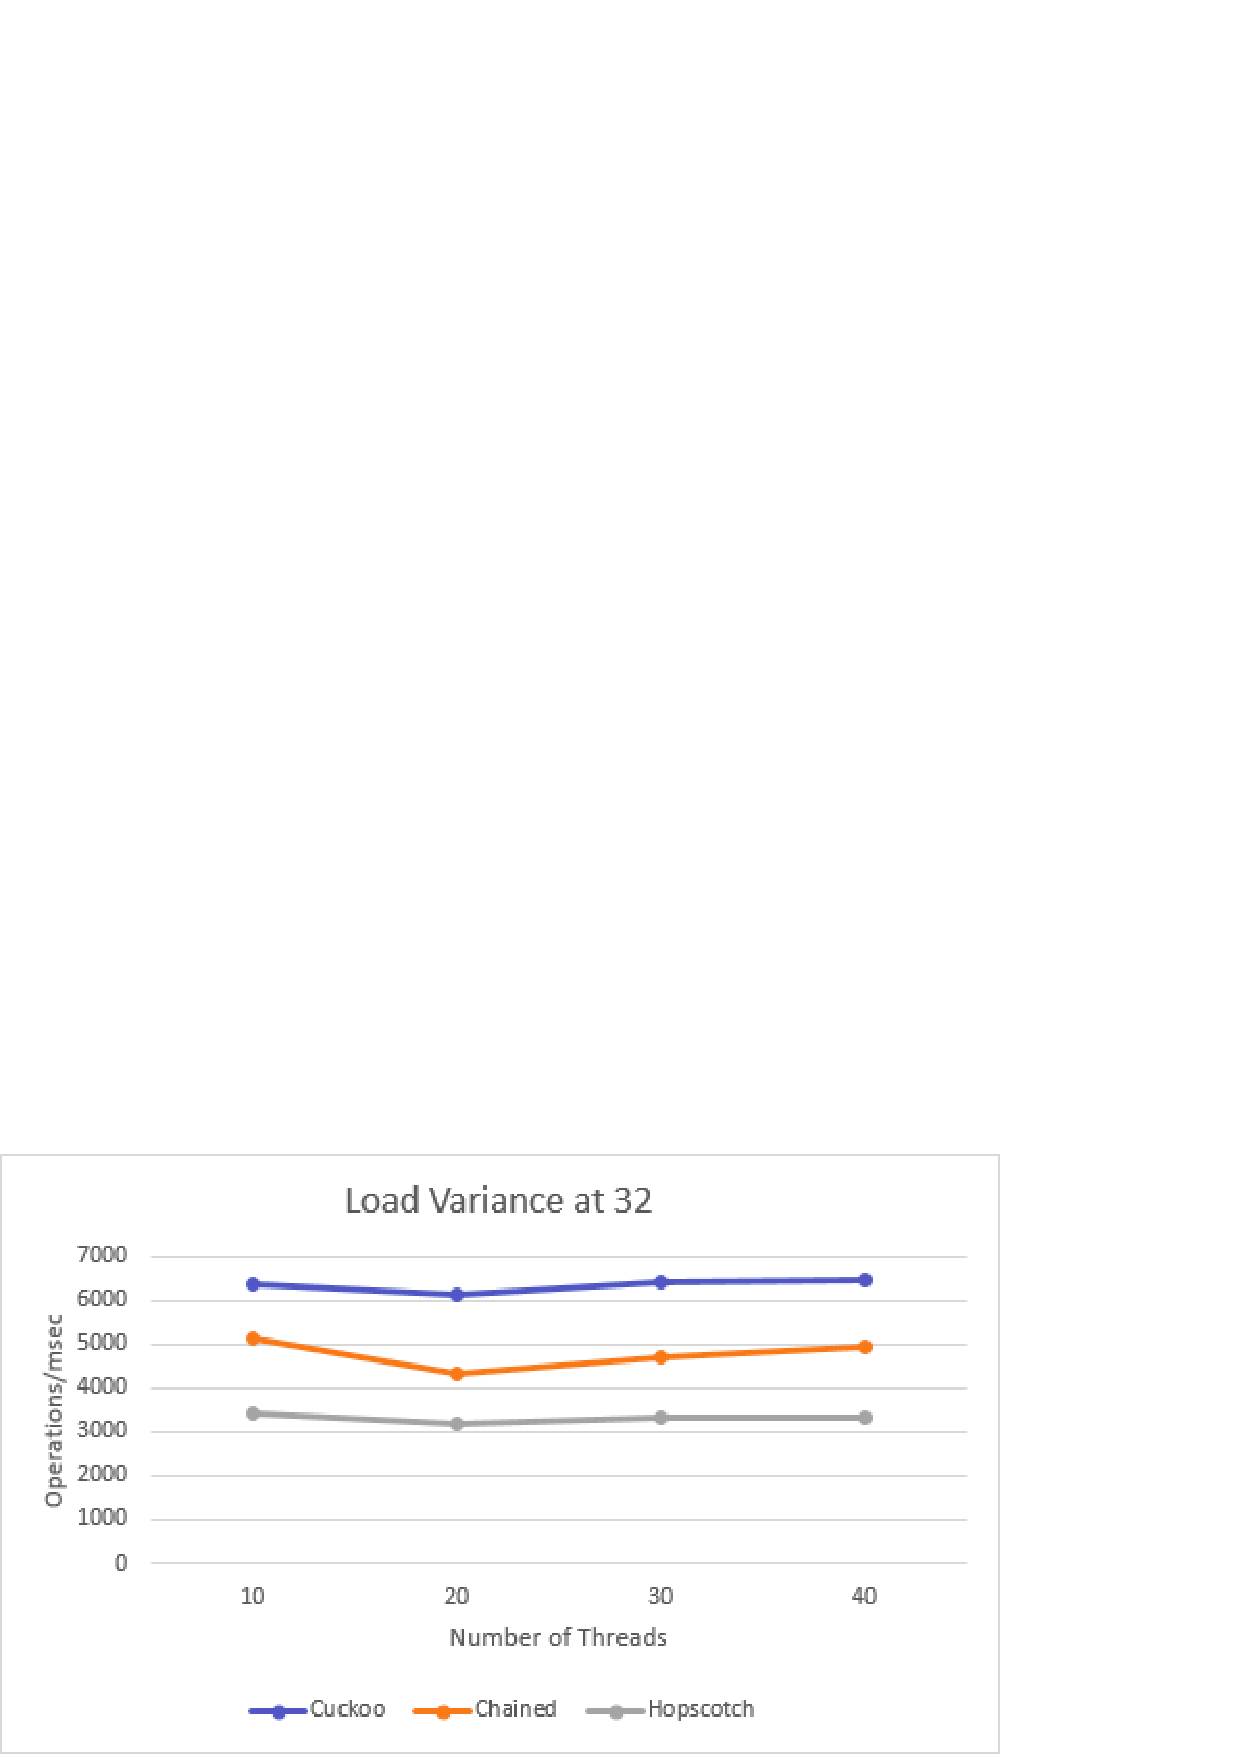
\includegraphics[width=2.9791in,height=1.7992in]{Report-img014.png} 


\bigskip

The top 4 figures present the throughput result of the hash tables in different distributions of actions. The bottom two
present the throughput at varying load factors. The most commonly found

distribution is 90\% search, 5\% insert and 5\% remove. Two others with more mutating operations: 80s/10i/10r and
60s/20i/20r were tested. \ One with more query-only operations. As it is well known that original cuckoo hashing does
not work well with load factors greater than 49\%, the max load factor used was 40\%. The concurrency increased up to
32 threads, the maximum number of concurrent hardware threads supported by the machines.

These results show that this new hashing algorithm outperforms the state of the art in most distribution, particularly
the most common ones, especially as the number of threads increases.

\section[Software Transactional Memory Implementation]{Software Transactional Memory Implementation}
This algorithm was also implemented using Rochester Transactional Memory.

The correctness is guaranteed by similar logic as the C++ implementation. Although there are some differences. Instead
of using compare and swap primitives, the nature of transactions being atomic were used. This was done because if any
memory involved in the transaction was altered by another thread the operation may fail as only one thread would be
allowed to continue. 

\subparagraph{Results}
The results are shown based on distributions of query frequencies of 94,90 and 80 were used, and transaction size, of
which sizes of 1,100, and 10 were used. The y-axis is throughput in terms of operations per millisecond and the x-axis
is the number of threads.

 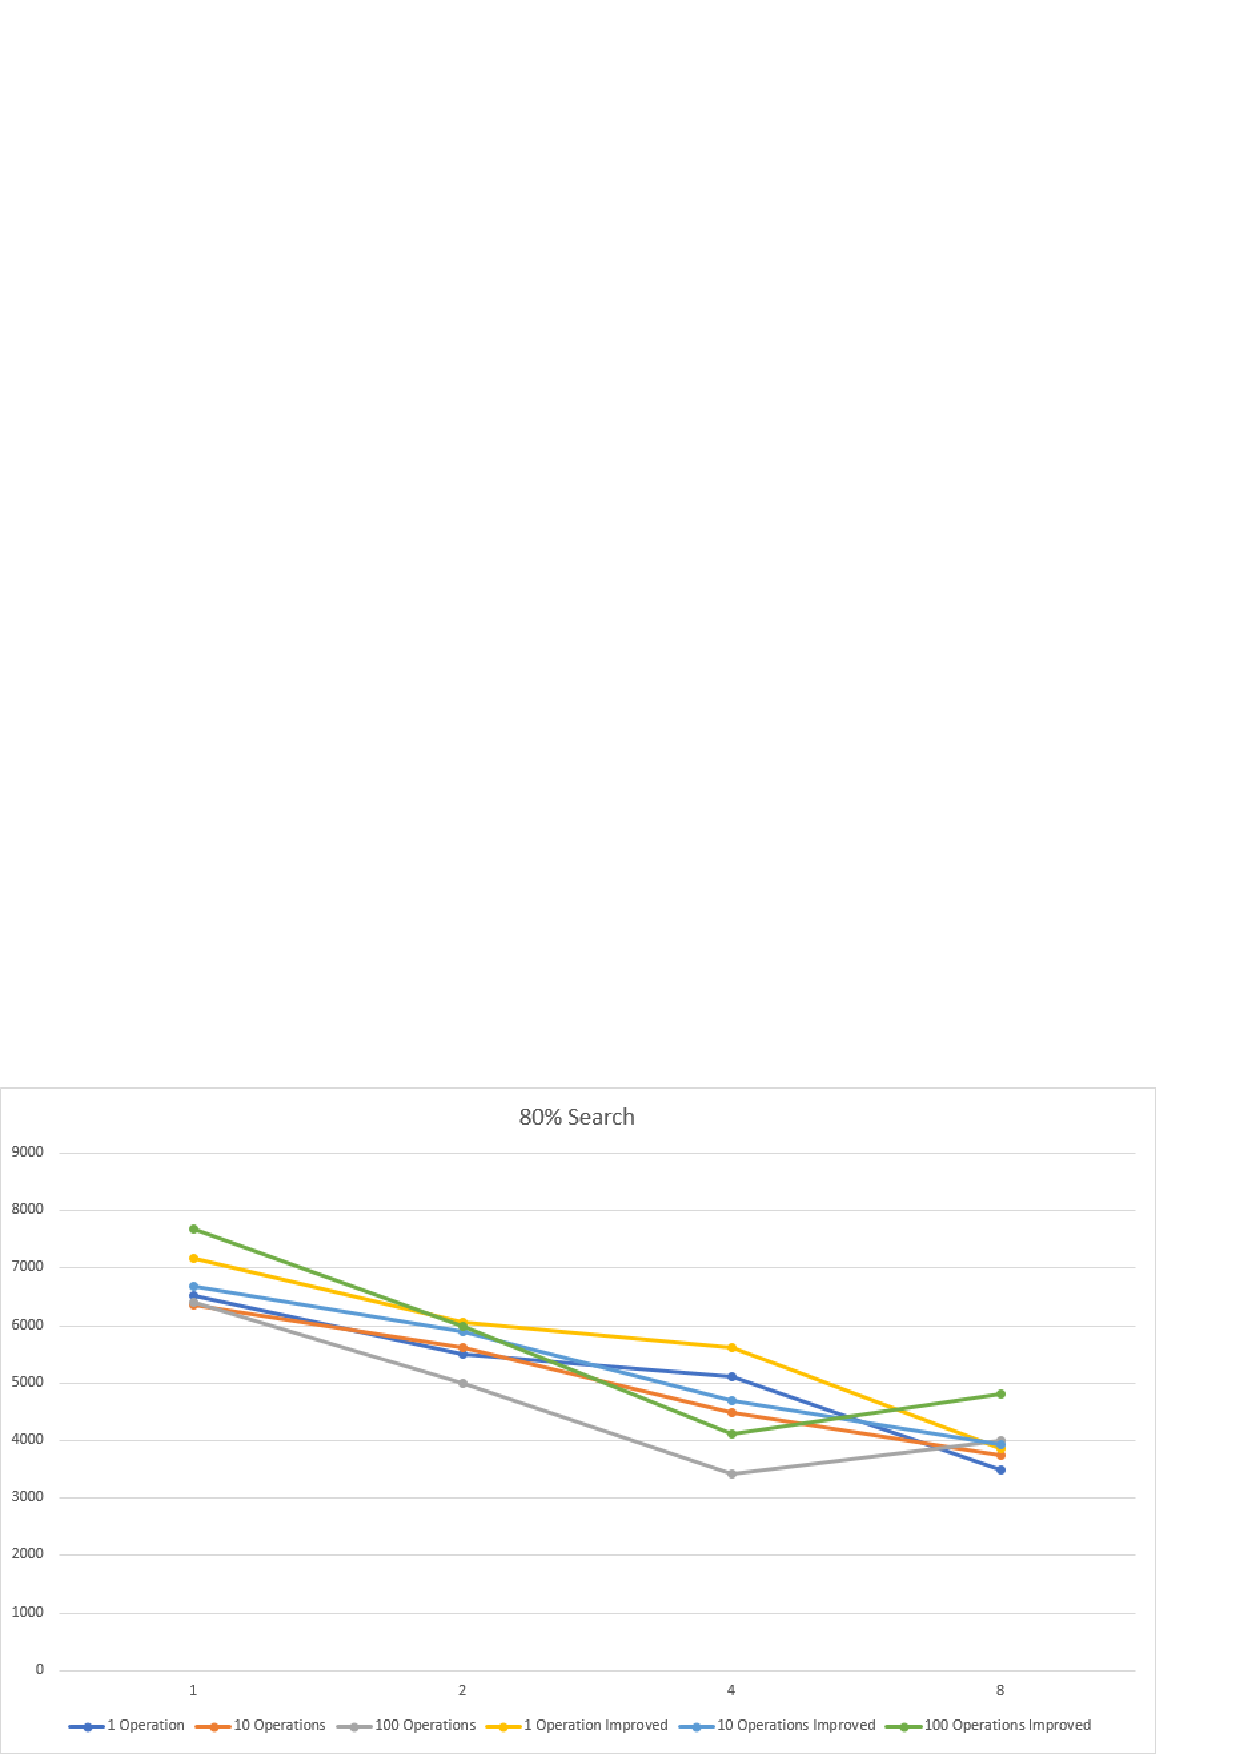
\includegraphics[width=2.9165in,height=1.6362in]{Report-img015.png} 
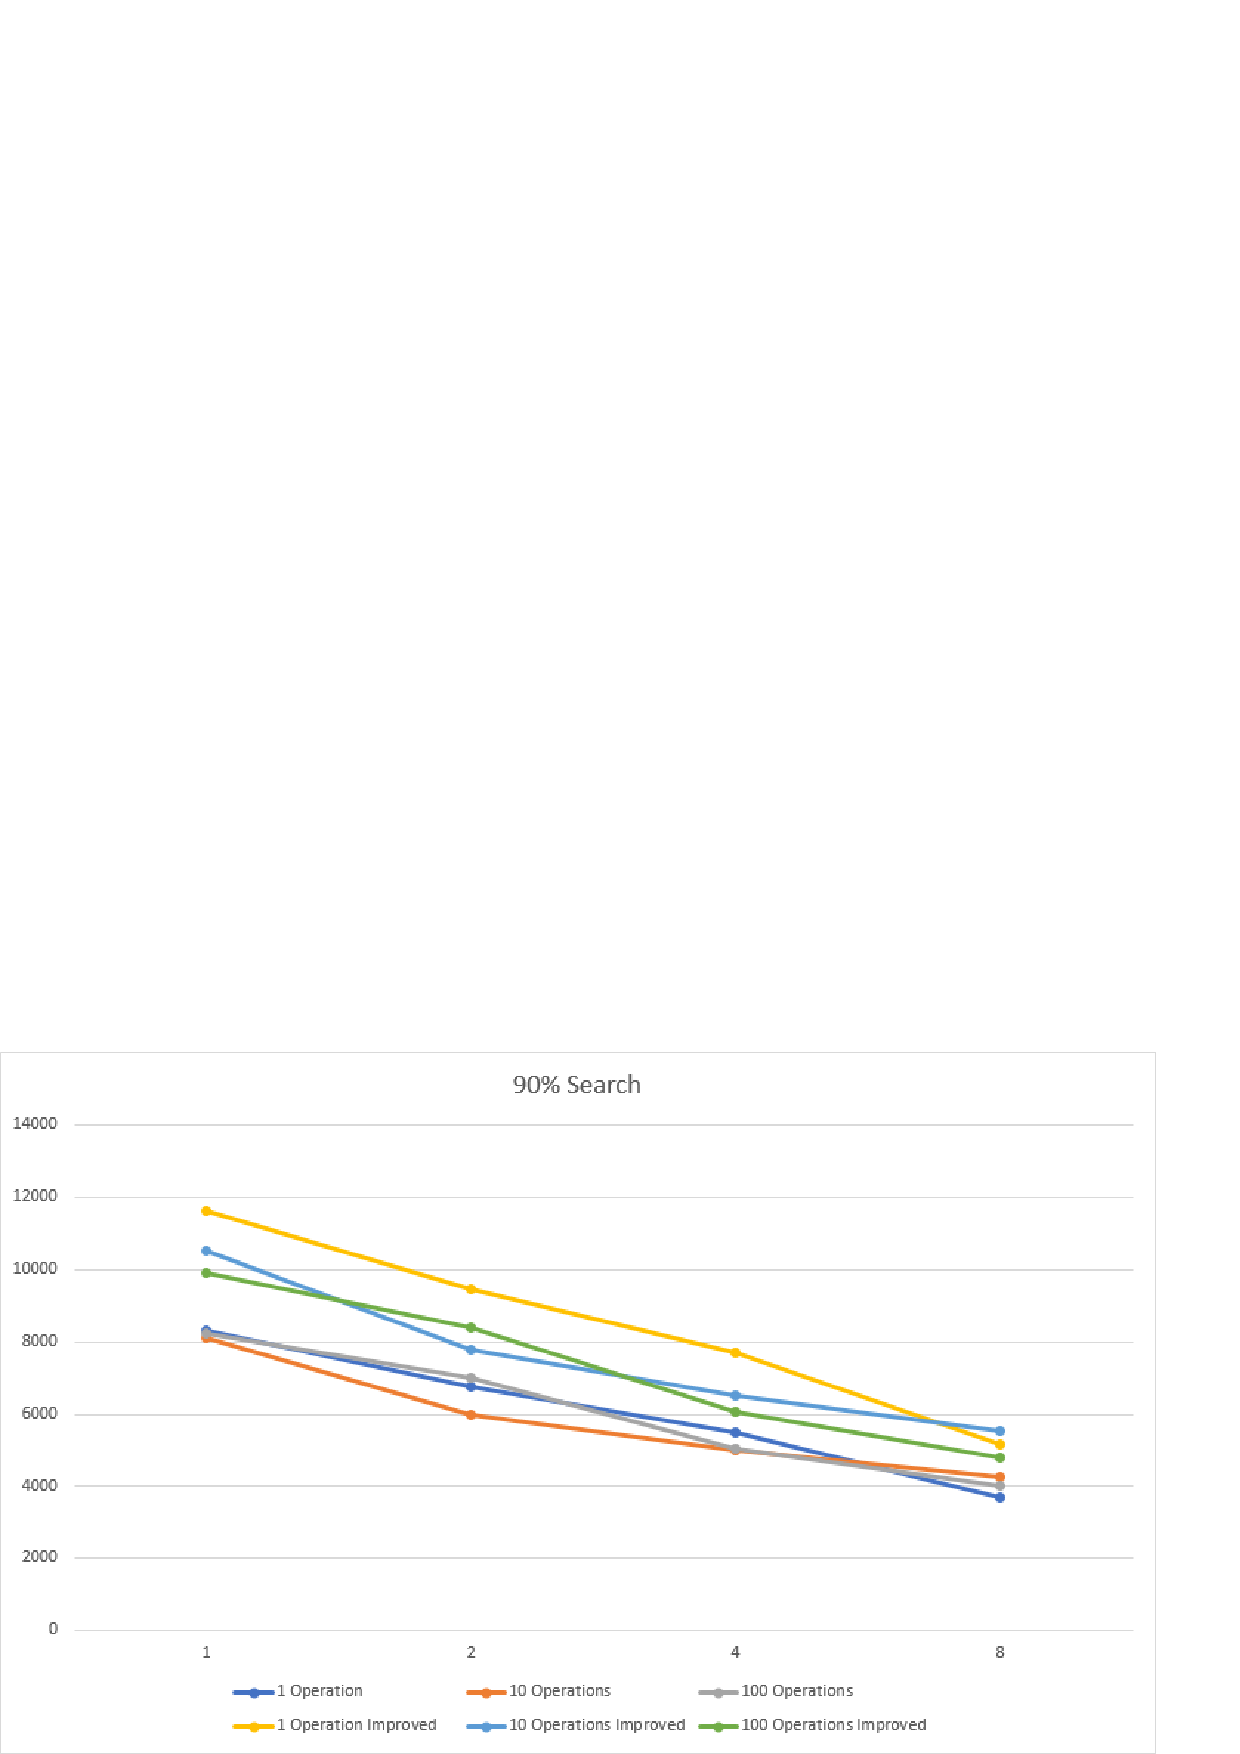
\includegraphics[width=2.8547in,height=1.6453in]{Report-img016.png} 

 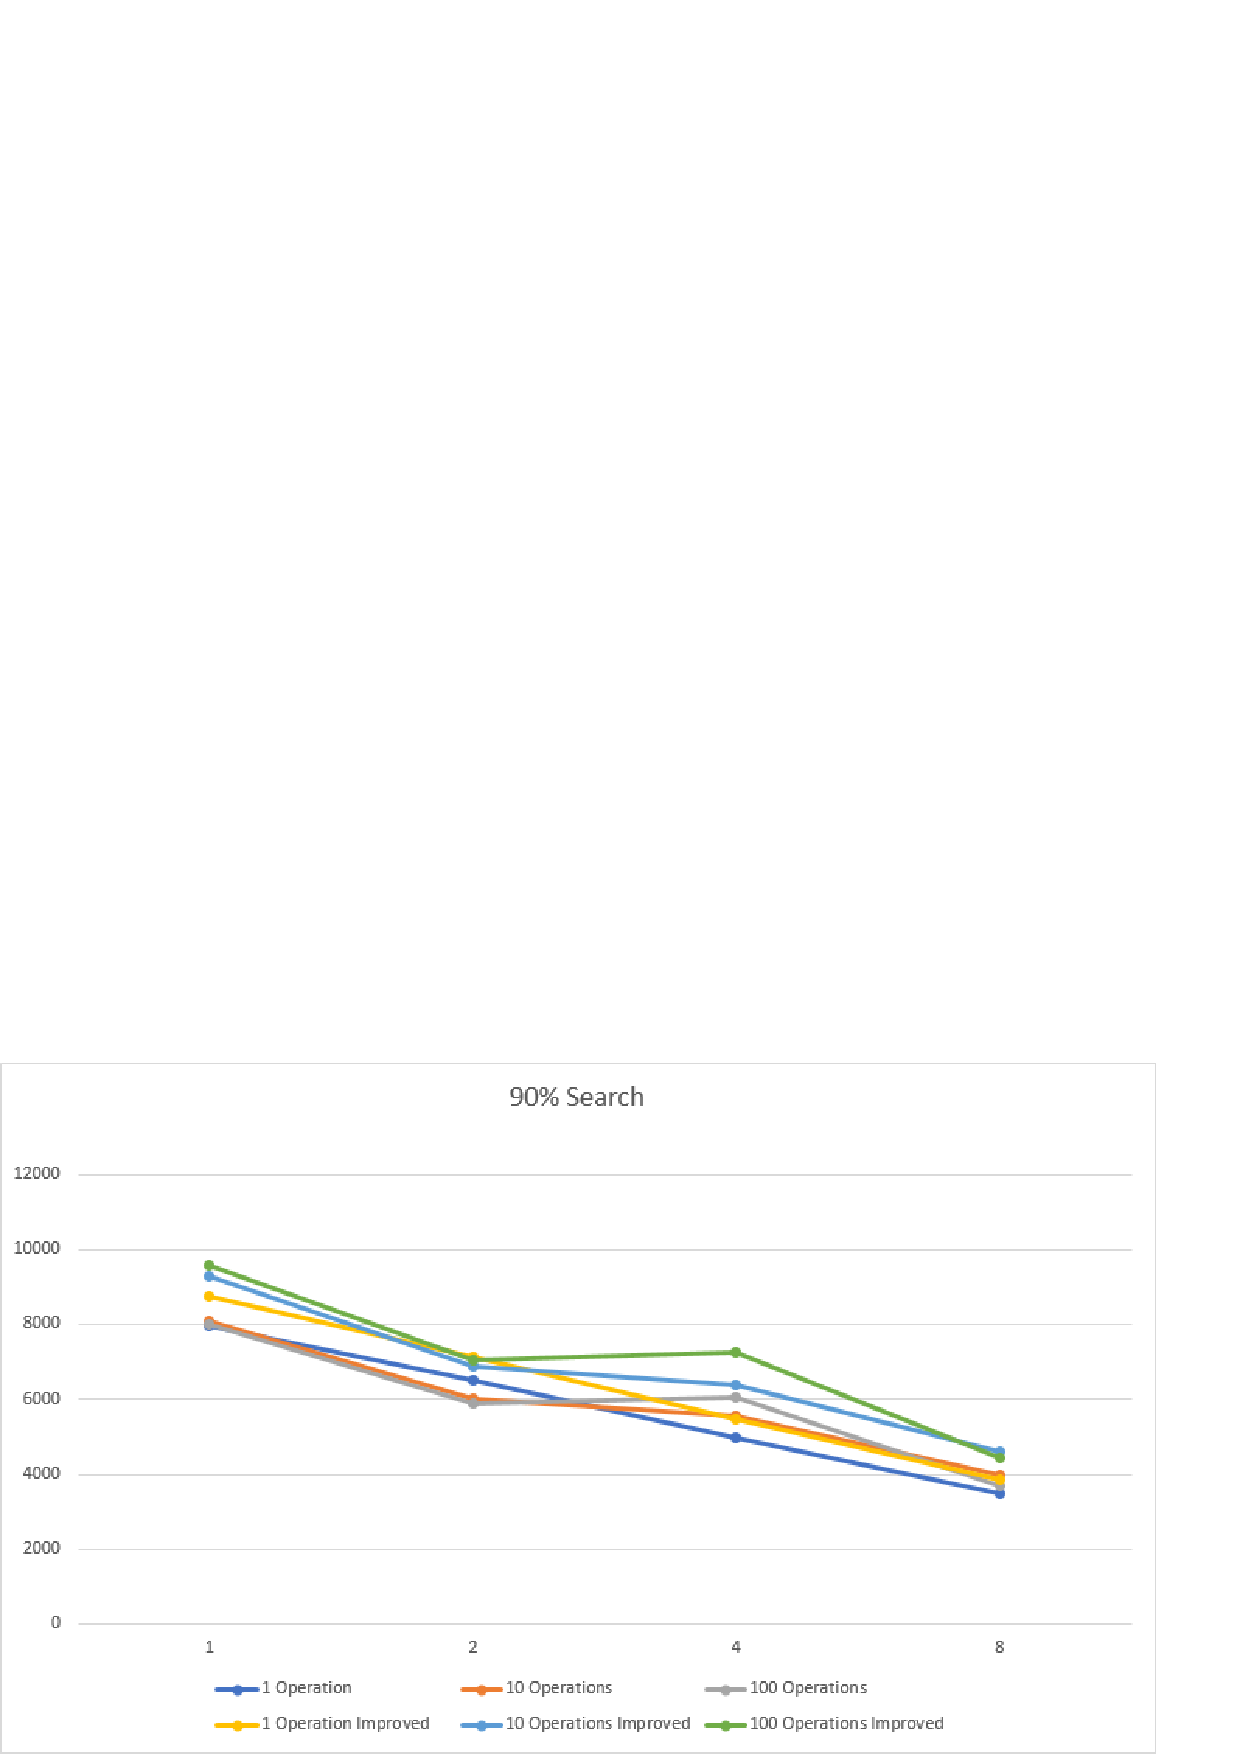
\includegraphics[width=2.8854in,height=1.7161in]{Report-img017.png} 
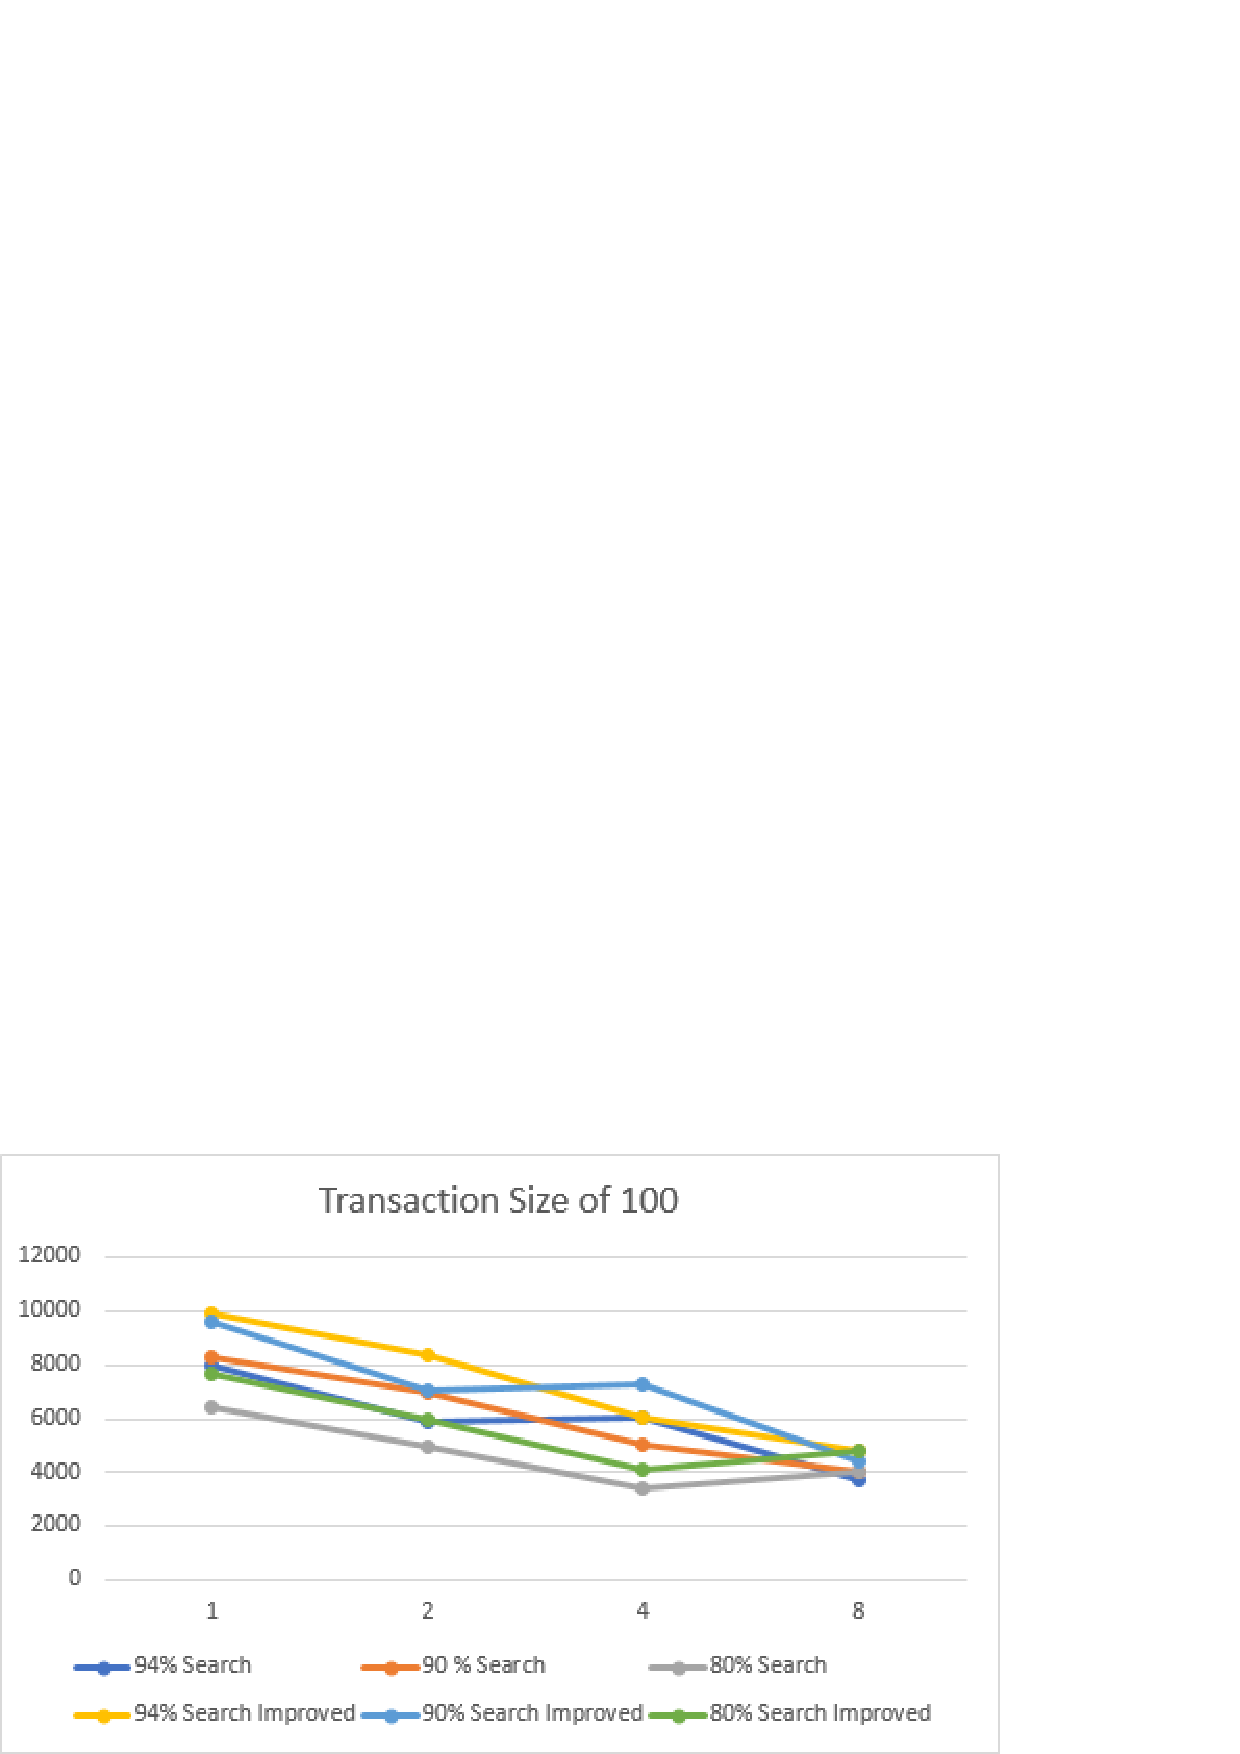
\includegraphics[width=3.0102in,height=1.8063in]{Report-img018.png} 


\bigskip


\bigskip

 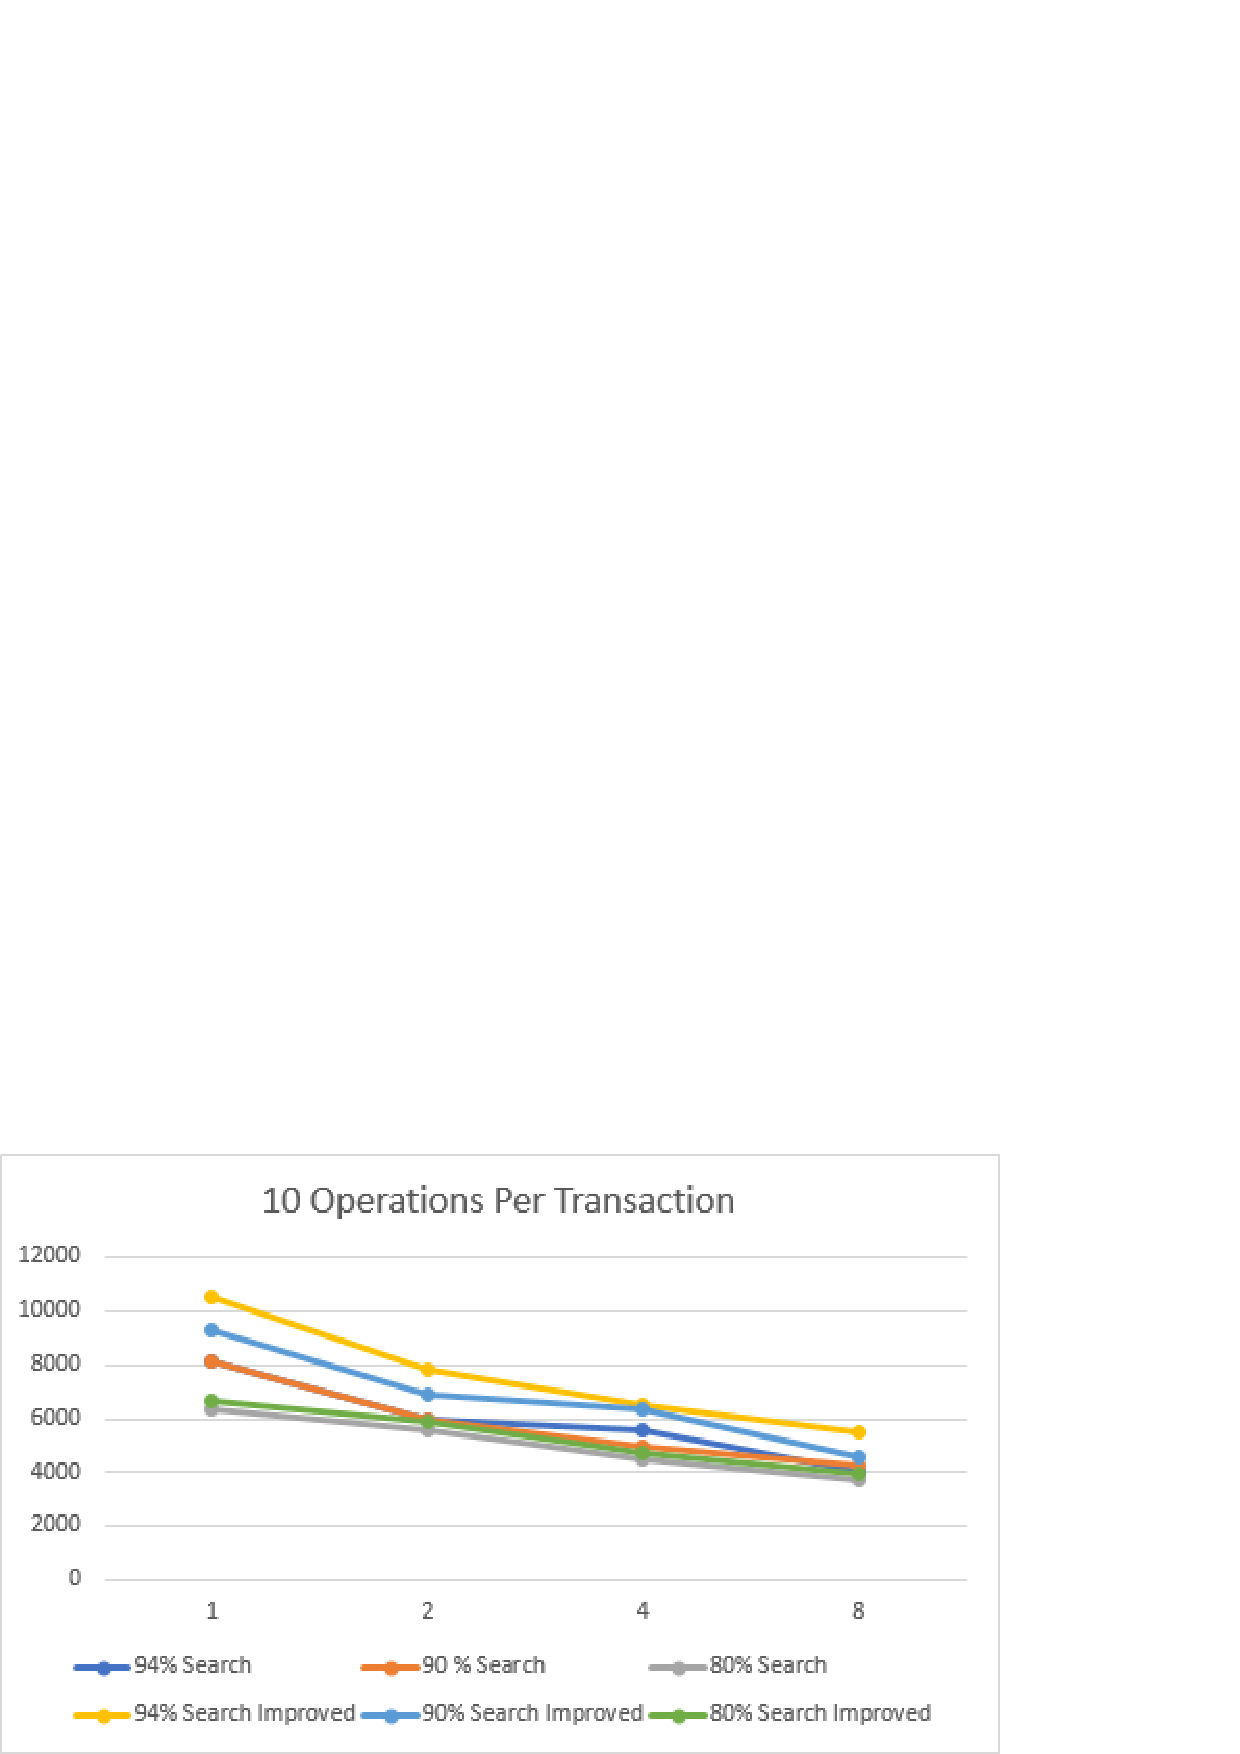
\includegraphics[width=2.9689in,height=1.7811in]{Report-img019.png} 
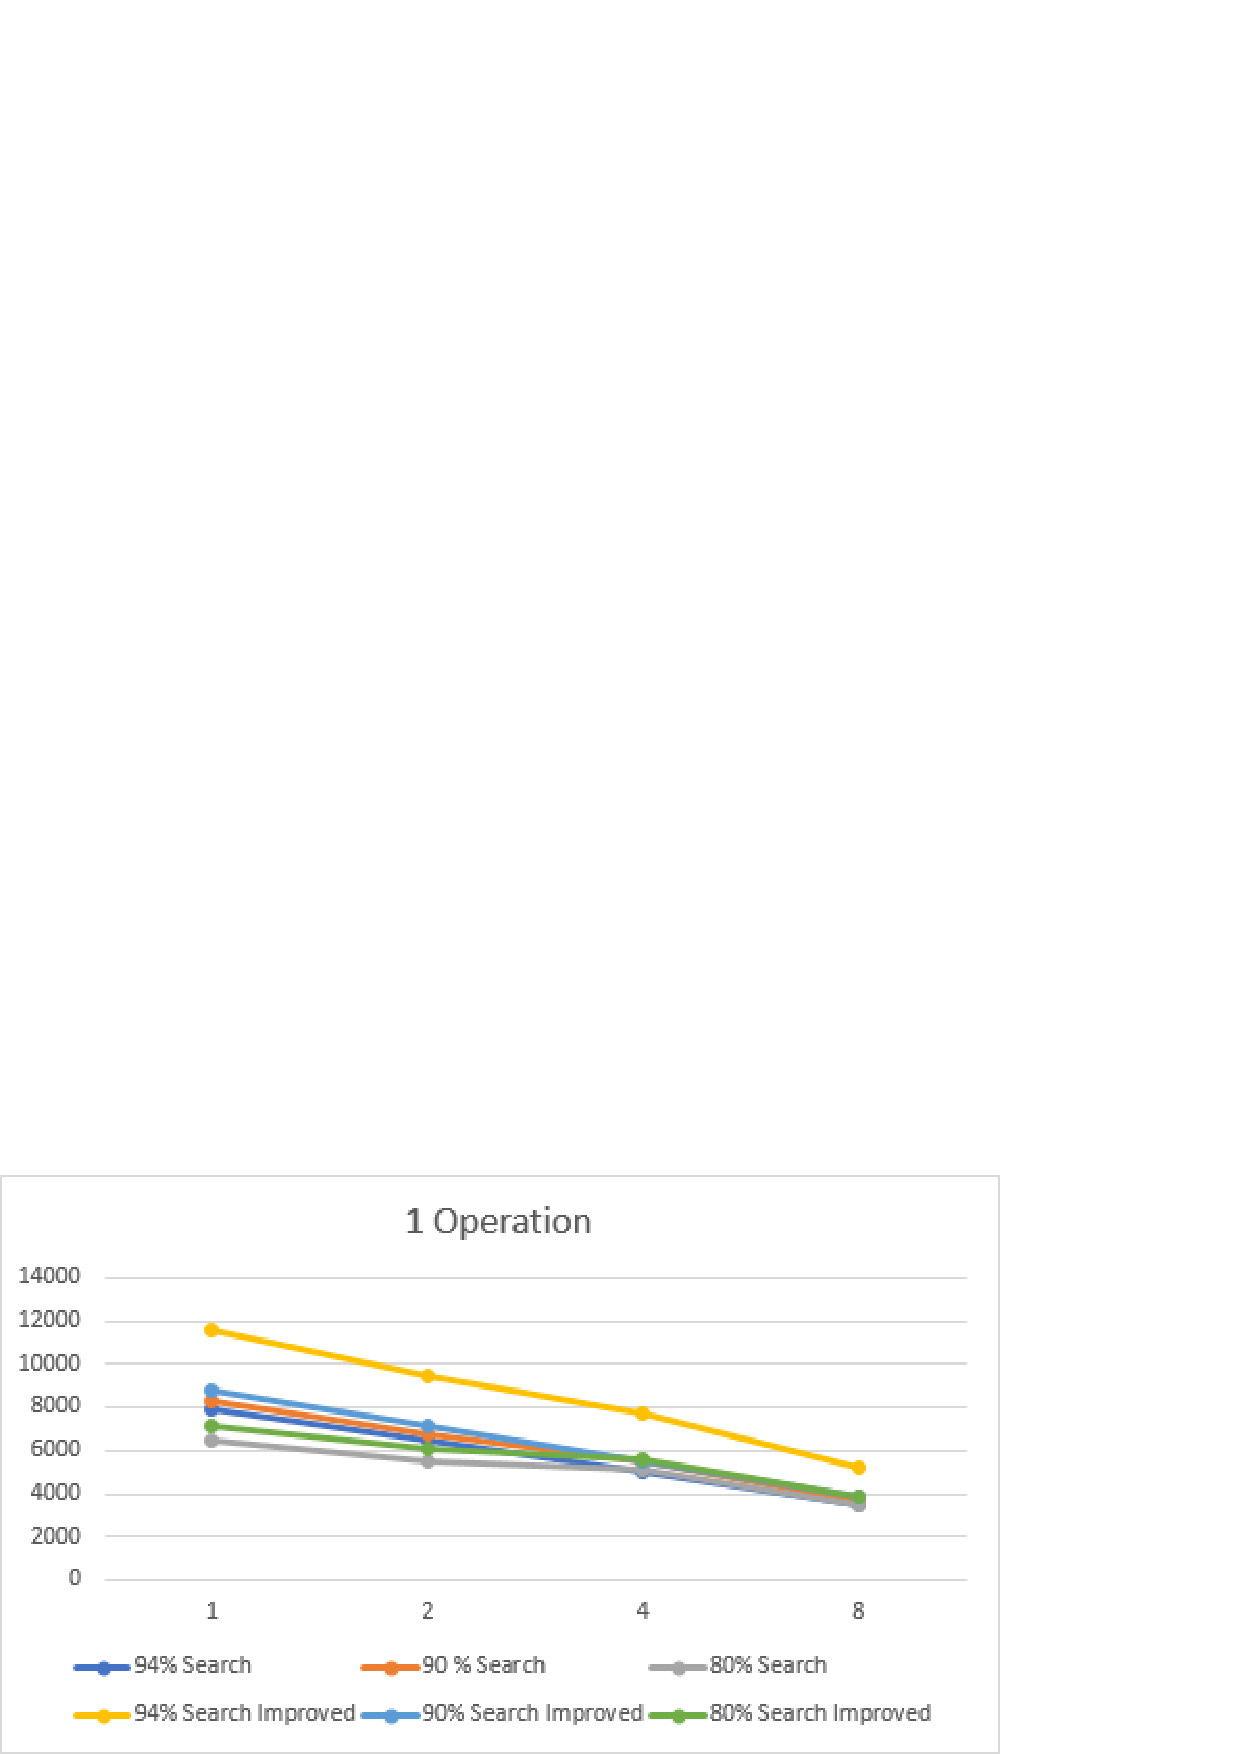
\includegraphics[width=2.9492in,height=1.7083in]{Report-img020.png} 


\bigskip


\bigskip

As the transaction size increase, the time were very similar and the number of aborted operations did increase as both
thread count and transaction sizes increased. The slight increase with increasing numbers of operations may be due to
aborting being quicker than completing a transaction. The throughput decreasing with increasing thread counts may be
due the sort of locking system that STM is based off of its reducing access to a control section. Modifications were
made to reduce the number of abortions such as not using compare and swap primitives. Another modification was to
replace the atomic compare and swap with a sort of compare and swap using transactional memory by reading and then
writing in a new value.


\bigskip

\subparagraph[Proof of STM]{Proof of STM}
Lemma 1: Search is linearizable

Proof: search only returns a value when one of the key e1, e2, e1b,e1c has an element that matches the key being
searched for and is linearized at that point. The second case is when search returns NOTFOUND. If there are
relocations, the search operation would not be majorly affected as it is not mutating the data.

Lemma 2: This locate operation is linearizable.


\bigskip

Lemma 3: The insert operation is linearizable.

Lemma 4: The remove operation is linearizable.

Theorem 1: The hashing algorithm is linearizable.

\section{Conclusion}
This algorithm uses atomic primitives which are widely available in modern computer systems. \ However, this new hashing
algorithm is not resizable and loses a lot of memory, even with proper memory management. We have performed experiments
that compares our algorithm with the efficient parallel hashing algorithms from the literature, in particular hopscotch
hashing and optimized lock-based chained hashing. The experiments show that our implementation is highly scalable and
perform as well or better than the other algorithms in all the access pattern scenarios.

\section[Acknowledgments]{Acknowledgments}
The author would like to acknowledge the authors of the original paper this was derived from, Nhan Nguyen and Philippas
Tsigas of Chalmers University of Technology Gothenburg, Sweden. \ the authors whos source code was used for the chained
and hopscotch hashing, Kaushik Basu and Jongsoo Park, respectively.

\subsection{References}
[1]Nhan Nguyen, Philippas Tsigas, {\textquotedbl}Lock-Free Cuckoo Hashing{\textquotedbl},~Distributed Computing Systems
(ICDCS) 2014 IEEE 34th International Conference on, pp. 627-636, 2014.

[2]Knuth, D. E.The art of computer programming, volume 1 (3rd ed.): fundamental algo-rithms. Addison Wesley Longman
Publishing Co., Inc., Redwood City, CA, USA, 1997

[3] M. Herlihy, N. Shavit, and M. Tzafrir, ``Hopscotch hashing,'' in The Proceedings of the 22nd International Symposium
on Distributed Computing (DISC), ser. LNCS, vol. 5218. Springer Berlin Heidelberg, 2008, pp. 350--364

[4]M. Herlihy and N. Shavit,The Art of Multiprocessor Pro-gramming.San Francisco, CA, USA: Morgan KaufmannPublishers
Inc., 2008

[5]M. M. Michael, ``High performance dynamic lock-free hashtables and list-based sets,'' inProceedings of the 14th
ACMSymposium on Parallel Algorithms and Architectures (SPAA).ACM, 2002, pp. 73--82.

[6] O. Shalev and N. Shavit, ``Split-ordered lists: Lock-free extensible hash tables,''Journal of the ACM, vol. 53, no.
3,pp. 379--405, May 2006.

[7]Nhan Nguyen, Philippas Tsigas, {\textquotedbl}Lock-Free Cuckoo Hashing{\textquotedbl},Chalmers University of
Technology, Department of Computer Science and Engineering, Tech. Rep 2014:03 January 2014.

[8]L. Lamport, ``Time, clocks, and the ordering of events in a

distributed system,'' Commun. ACM, vol. 21, no. 7, pp. 558--

565, Jul. 1978.


\bigskip
\end{document}
